\chapter{Cryo-EM and cryo-ET}

In this chapter, I describe the role of cryo-EM and cryo-ET in the field of structural biology, explain their fundamentals, and discuss advantages and limitations.

Structural biologists employ several techinques to understand the structure and function of biomolecular systems, typically proteins, nucleic acids and their ligands.
Arguably, the three giants in the field are X-ray crystallography, Nuclear Magnetic Resonance (NMR) and cryo-electron microscopy (cryo-EM), with several other techniques playing complementary, more specialized or niche roles (such as mass spectroscopy, neutron scattering or small-angle scattering).
Each technique has pros and cons, making it suited to different samples and applications.

In X-Ray crystallography --- in many ways the predecessor to cryo-EM as all-purpose structural biology technique --- crystals are grown from the sample of interest; the crystals are then illuminated by an X-ray beam, and the diffraction pattern thus created can be detected and used to reconstruct the three-dimensional (3D) structure of the sample.
Thanks to the short wavelength of X-rays --- as opposed to visible light --- it is possible to localize the positions of atoms with sub-angstrom precision.
X-ray crystallography has played a major role in the development of structural biology, and is still the primary source of protein structures on the Protein Data Bank~\cite{bermanProteinDataBank2000,bermanAnnouncingWorldwideProtein2003}.
However, the need for crystallization poses a few limits.
The crystallization procedure is often hard to devise and reproduce, extending the time and resources needed for sample preparation.
Moreover, the resulting crystal "forces" the sample into a crystalline lattice, often with biologically irrelevant chemical states, restricting the conformational freedom of the molecule and limiting the biological significance of the obtained structures~\cite{ravikumarComparisonSidechainDispersion2022}.

\section[Cryo-EM and SPA]{Cryo-electron microscopy and single particle analysis}

Cryo-EM improves on these aspects by forgoing crystallization in favor of sample vitrification, which allows to capture the sample in near-native state. This requires analysing many individual particles at different orientations, in a procedure known as single particle analysis (SPA).

In simple terms, the electron microscope works by shooting a coherent electron beam at the sample, and using a camera to detect the scattered electrons and form an image.
Thanks to the small wavelength of electrons, cryo-EM can reach much higher resolution than light microscopy; however, it presents unique challenges and limitations that its more familiar light-based counterpart does not.

In the last decade, the development of direct electron detectors made it possible to reach atomic resolutions, jump-starting to the so-called resolution revolution and the rise of cryo-EM as one of the primary methods for high resolution structure determination~\cite{faruqiCCDDetectorsHighresolution2000}.

Differently from light-microscopy, which relies on amplitude contrast for image formation, the electron microscope uses phase contrast, which is caused by elastic scattering events affecting the electrons traversing the sample.
Some electrons, however, are inelastically scattered; these electrons are no longer coherent, and therefore add to the noise of the image.
Increasing the electron dose can help improve the signal-to-noise ratio (SNR), but comes at the cost of radiation damage, which denatures the sample and rapidly destroy high-resolution information.
For these reasons, a significant limitation --- and thus optimization target --- of cryo-EM is the low SNR.

The cryo-EM workflow is well established, and usually consists of the same principal components: sample preparation and vitrification, data collection, preprocessing (cleaning, motion and CTF correction), particle picking and classification, three-dimensional (3D) reconstruction, and model building.
This section describes such typical workflow, expanding on the theoretical bases surrounding each step.

\subsection{Sample preparation}
Cryo-EM samples for SPA are usually prepared in vitro by expressing ad purifying the protein or complex of interest to create a minimal system.
Sample concentration and purity are important variables to control, as they will affect vitrification and data processing complexity.
The sample solution is then deposited on a cryo-em grid and vitrified via plunge freezing in liquid ethane or other methods (\autoref{fig:em_plunge_freezing})~\cite{dubochetCryoelectronMicroscopyVitrified1988}.
Vitrification allows to fixate the sample at near-native, hydrated conditions while avoiding the formation of crystalline ice, which would damage the sample.
When vitrifying, the thickness of the ice is crucial: a thinner layer will results in fewer inelastically scattered electrons during data collection and better SNR.
However, too-thin ice can crack and increase issues with preferential orientation or particle distribution.

\begin{figure}[ht]
    \centering
    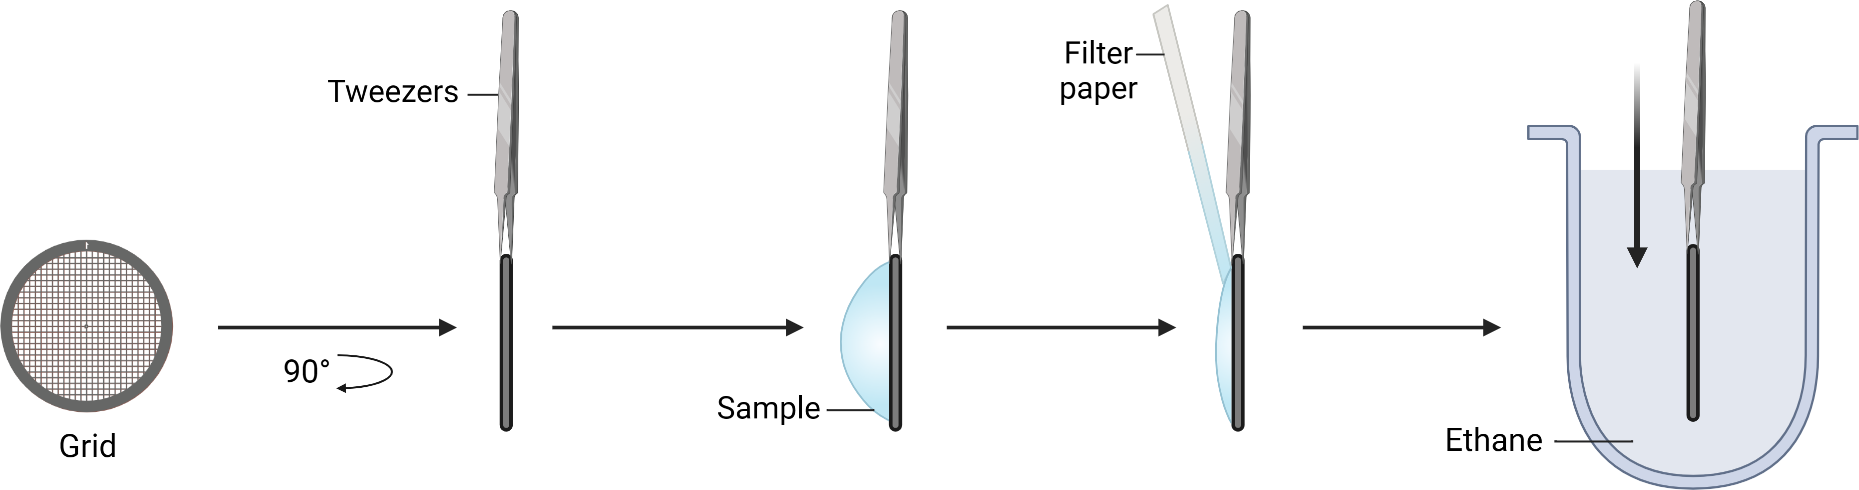
\includegraphics[width=\textwidth]{introduction/plunge_freezing.png}
    \caption[Vitrification via plunge freezing]{Typical vitrification procedure via plunge freezing. A drop of sample is placed on the grid, blotted with a filter paper to reduce its thickness to a thin layer, and then plunged into liquid ethane. Figure adapted from \citet{chungNobelPrizeChemistry2017}.}
    \label{fig:em_plunge_freezing}
\end{figure}

TODO: talk about tilted data collection and/or easy-grid, chameleon and vitrojet (but later)

\subsubsection{Preferential orientation}
A common issue with sample preparation for cryo-EM is non-uniform orientation distribution of the protein in the vitrified sample, often due to particles being adsorbed to the air-water interface~\cite{nobleRoutineSingleParticle2018}.

Strong preferential orientation may completely preclude the ability to do a 3D reconstruction, due to the lack of a wide distribution of orientations (see \fullref{em_reconstruction}).
When this problem arises, there are a few ways to tackle it during sample preparation.
The most common is the addition of small amounts of detergents to occupy the air-water interface and prevent particles from preferentially orienting hydrophobic surfaces out of the water.
Other methods are a bit more involved, such as the use of functionalized graphene grids~\cite{luFunctionalizedGrapheneGrids2022}, streptavidin-coated affinity support grids~\cite{crucifixImmobilizationBiotinylatedDNA2004,hanLongShelflifeStreptavidin2016}, but can offer more control over the orientation of the particles in the sample.

\subsection{Data collection}
The vitrified sample is loaded into the electron microscope (under cryogenic conditions and vacuum, in order to maintain the sample vitrified and uncontaminated), and suitable positions on the grid are chosen for imaging, prioritizing for: presence of the target protein or complex, fewer contaminations, and lower ice thickness.
In modern workflows and software, this step and the subsequent data collection are increasingly automated, allowing for higher throughput (up to several thousand images per day) and lower human intervention~\cite{schorbSoftwareToolsAutomated2019}.

During collection, the sample stage and electron beam are moved to each position to collect micrographs.
At each position, a short movie is recorded, consisting of a few low-dose, short-exposure frames: this allows to reduce the blur caused by intra-frame motion (induced by external factors among which the electron beam itself); the frames will later be aligned and averaged to produce a single higher-contrast image.
Direct detectors are therefore crucial not only for their raw improvement in achievable resolution, but also for their high speed, contributing to the reduction of yet another source of noise.

An important concept to be mindful of when setting up a data collection is defocus; in order to better understand how defocus affects later processing steps, we first need to understand image formation in the electron microscope, and the importance of estimating and correcting the Contrast Transfer Function (CTF).

\subsubsection{Image formation}

In electron microscopy, image contrast derives almost entirely from phase contrast.
The electron beam generated by the microscope is initially coherent, that is the phases of all the electrons in the beam are correlated.
When electrons traverse the sample, they have a chance to undergo elastic scattering; this results in a shift in the electron's phase, leading to interference with the unscattered wave at the image plane (\autoref{fig:em_image_formation}).
It's this interference that create phase contrast, which the camera detects to generate the image.

Some electrons are also inelastically scattered: these electrons lose energy and coherence, and are therefore adding to the noise of the image because the lenses no longer focus them to the right place.
To mitigate this effect, inelastically scattered electrons are filtered out using an energy filter, which removes electrons with energy that differs significantly from the unscattered ones (\autoref{fig:em_image_formation}).

Inelastic scattering is also the source of radiation damage: the energy lost by these electrons is transferred to the sample, denaturing and deforming it and thus affecting SRN.

Sample thickness is of crucial importance for image formation: higher thickness results in higher chance for collision, increasing the chance of inelastic scatterings.
Additionally, a thicker sample may result in multiple elastic scattering events, which further alter the phase but cannot be distinguished from single scattering events, contributing to image noise.

\begin{figure}[ht]
    \centering
    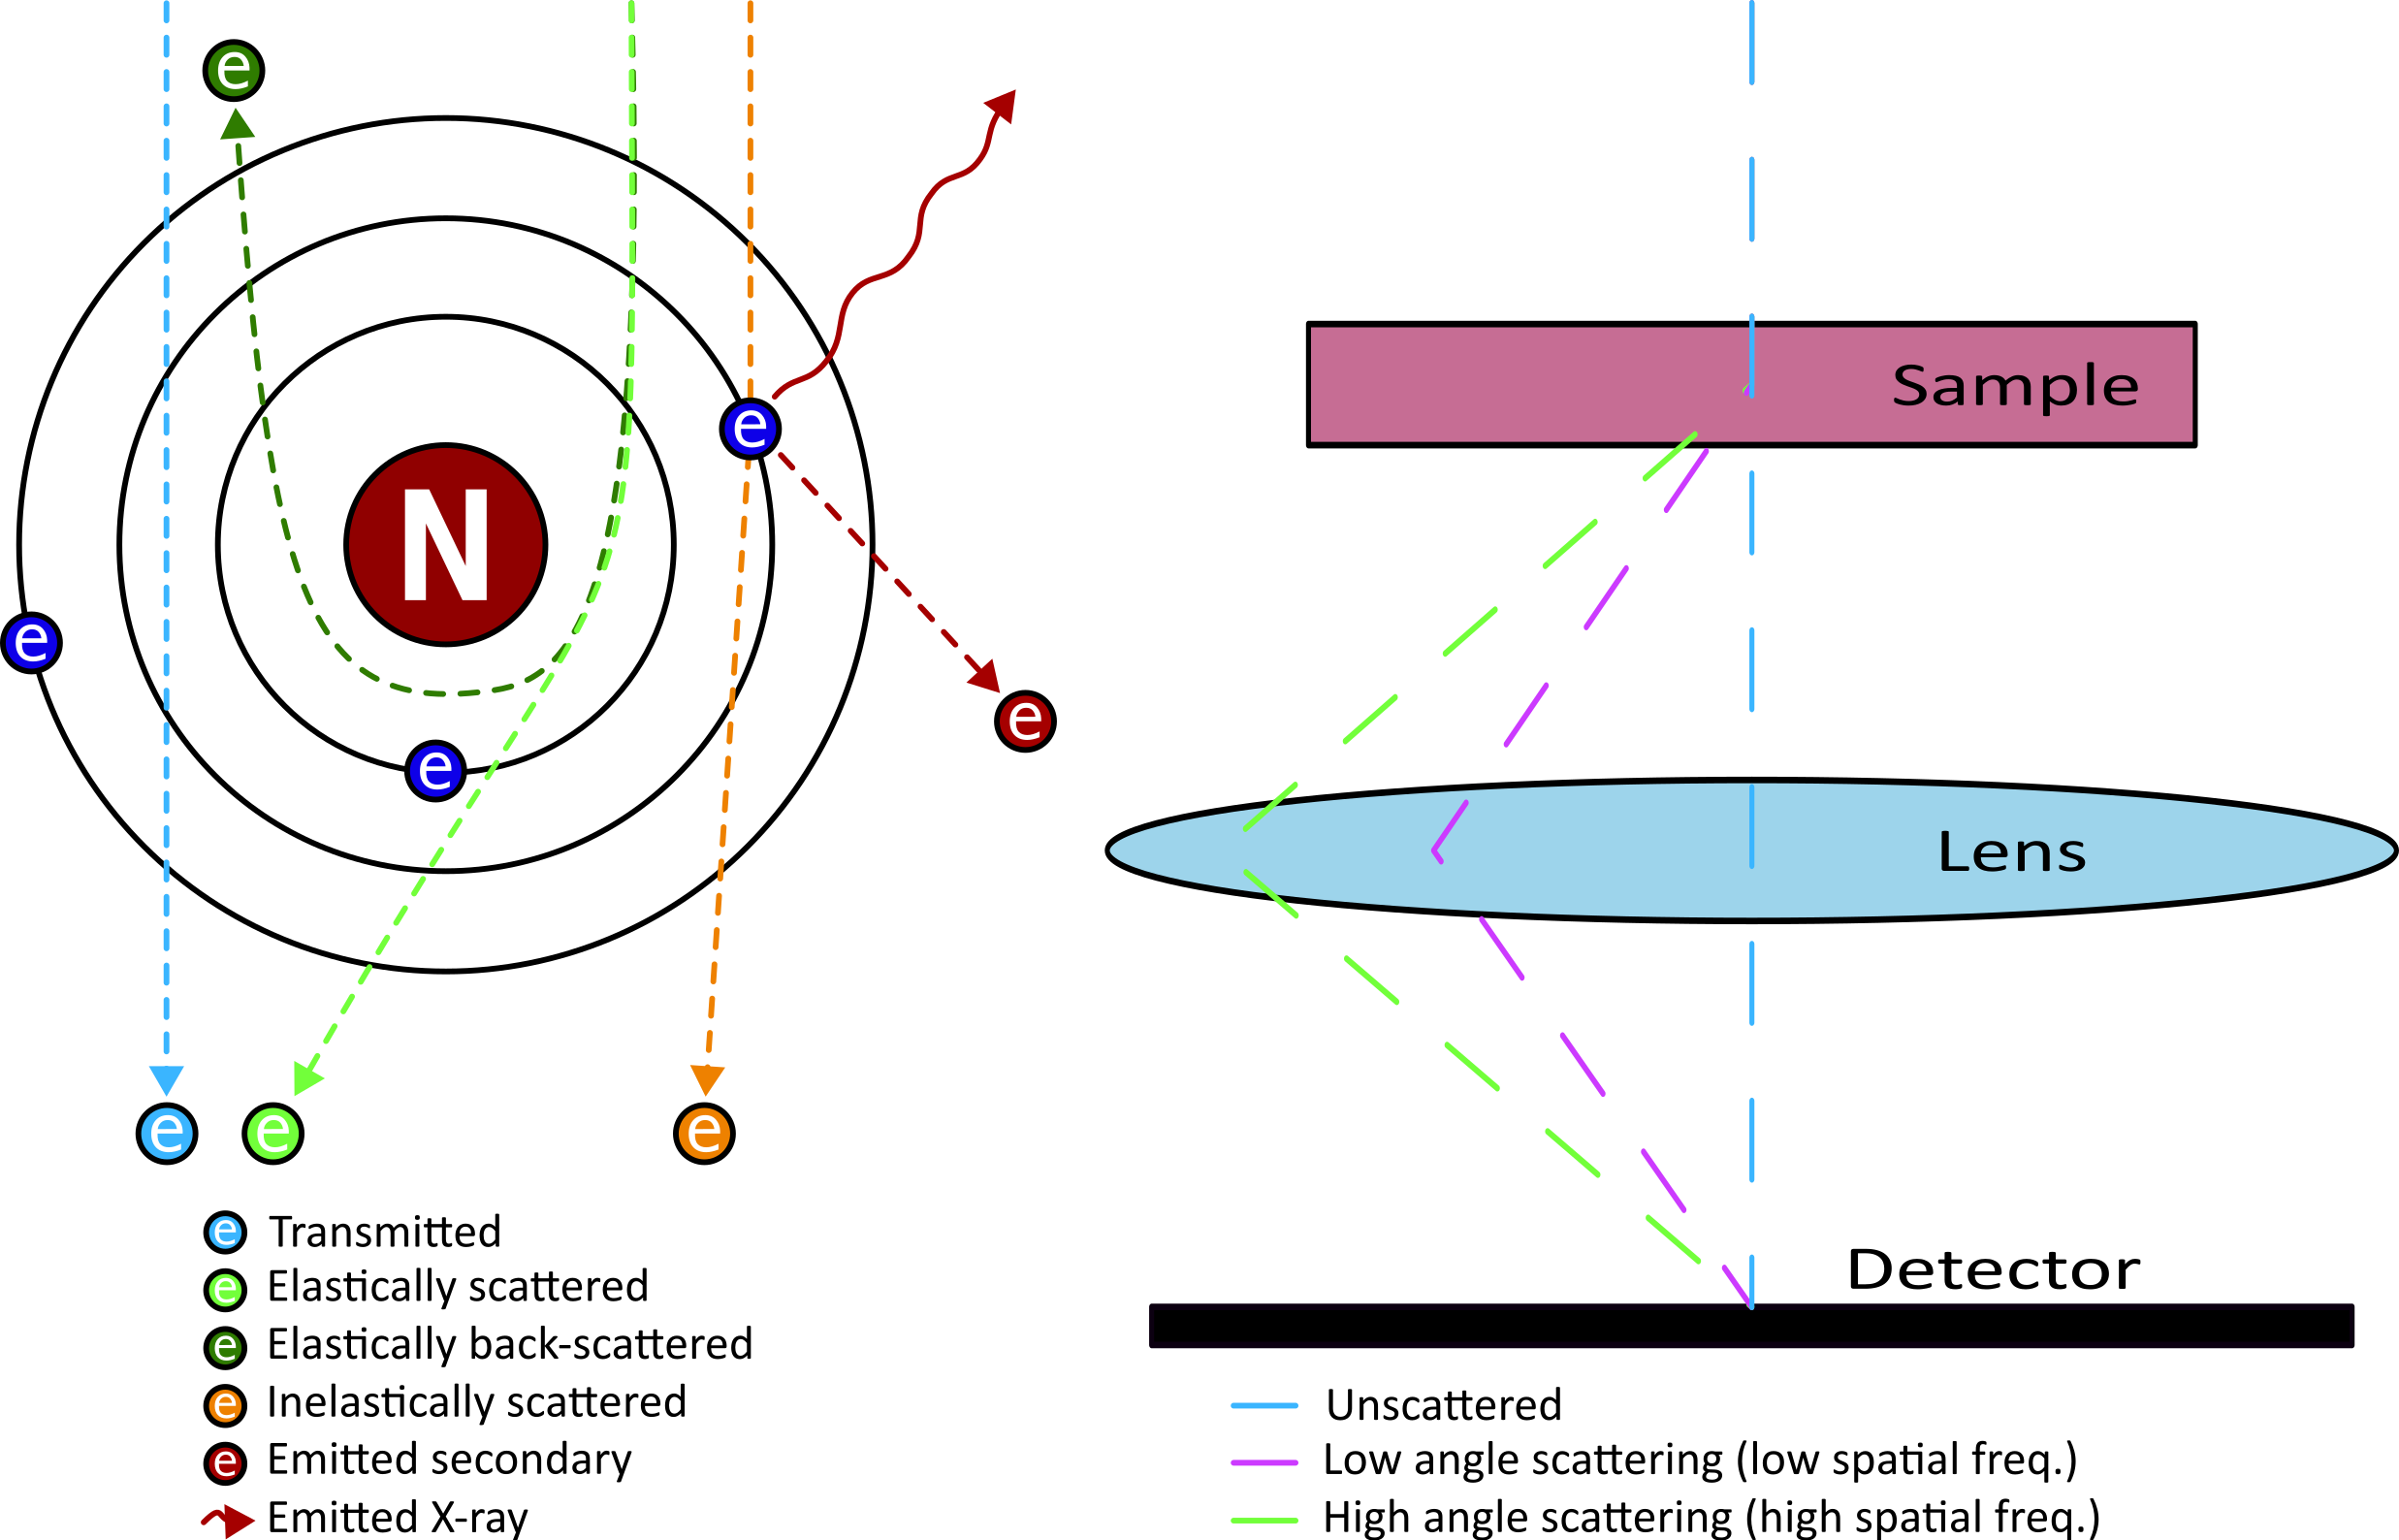
\includegraphics[width=\textwidth]{introduction/scattering.png}
    \caption[Image formation]{Electron scattering and diffraction are the physical processes at the core of cryo-EM image formation. Electrons can scatter in several different ways (left), but only elastic scattering contributes to image formation via phase contrast with the trasmitted electrons. Features contained in the sample that present different spatial frequencies result in scattering at different angles (right); depending on the difference in path travelled and the wavelength of the electron beam, this results in interference between differently scattered waves. In this figure where wave oscillations are visualized as dashed lines, we can see that the unscattered and low-angle scattered waves result in constructive interference, while the high-angle scattered interferes destructively.}
    \label{fig:em_image_formation}
\end{figure}

\subsubsection{Contrast Transfer Function}\label{em_ctf}
The shift induced in the phase of the electron wave by elastic scattering events is closely related to the spatial frequency of features in the sample: smaller details such as the relative positioning of neighboring \alpha-helices, which contain information at higher spatial frequency, will scatter to higher angles; bigger features such as biological membranes will scatter to lower angles.
Depending on the angle, the interference at the image plane will be constructive or destructive, resulting in certain spatial frequencies being dampened or lost.

The CTF is a function that describes exactly this: how signal is transmitted through the sample and onto the image, as a function of spatial frequency.
Where the CTF reaches a value of \num{0}, no signal is transferred; a value of \num{1}, on the other hand, is a perfect signal transfer.

The CTF has a close relationship with the fourier transform (FT) of a micrograph: the 1D rotational average of the power spectrum (PS) of the image (the square of the amplitude of the FT of the image) forms the curve used to estimate the CTF (\autoref{fig:em_ctf_defocus}).
An ideal sample with a uniform distribution of spatial frequencies would produce a 1D PS identical to its theoretical CTF.

The CTF is usually described as composed of two main elements.
The first one is a sinusoidal component caused by the periodicity of destructive and constructive interference of electron phases at different spatial fequencies.
It is visible in the PS of cryo-em images as a set of concentric rings called Thon rings (\autoref{fig:em_ctf_defocus_2d}).
The exact shape of the Thon rings depends on several factors, first among which the defocus: changing defocus affects the oscillation frequency, thus shifting the zeros of the CTF and boosting or nullifying different spatial frequencies (\autoref{fig:em_ctf_defocus_1d}).

\begin{figure}[ht]
    \centering
    \begin{subfigure}{.6\textwidth}
        \centering
        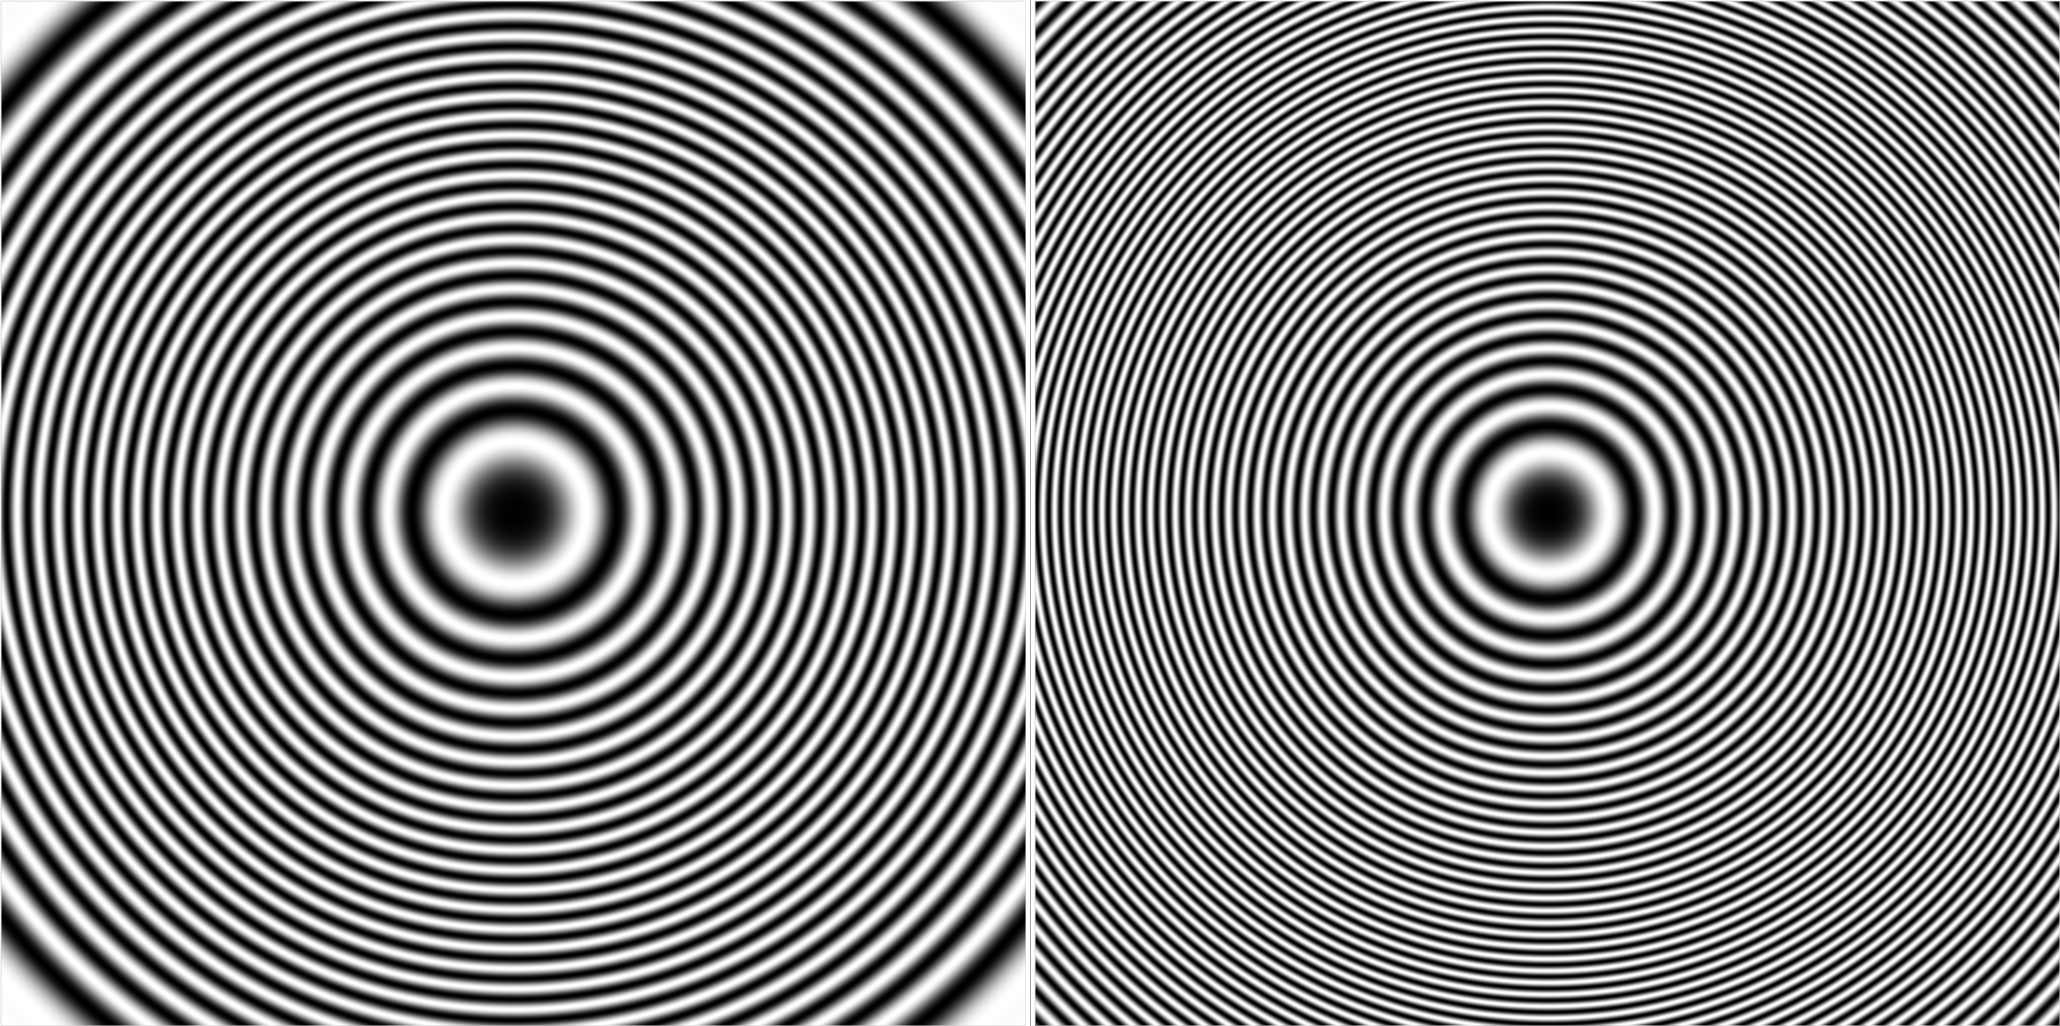
\includegraphics[width=\textwidth]{introduction/ctf_defocus_2d.png}
        \caption{2D power spectrum ($CTF^2$).}
        \label{fig:em_ctf_defocus_2d}
    \end{subfigure}%

    \begin{subfigure}{\textwidth}
        \centering
        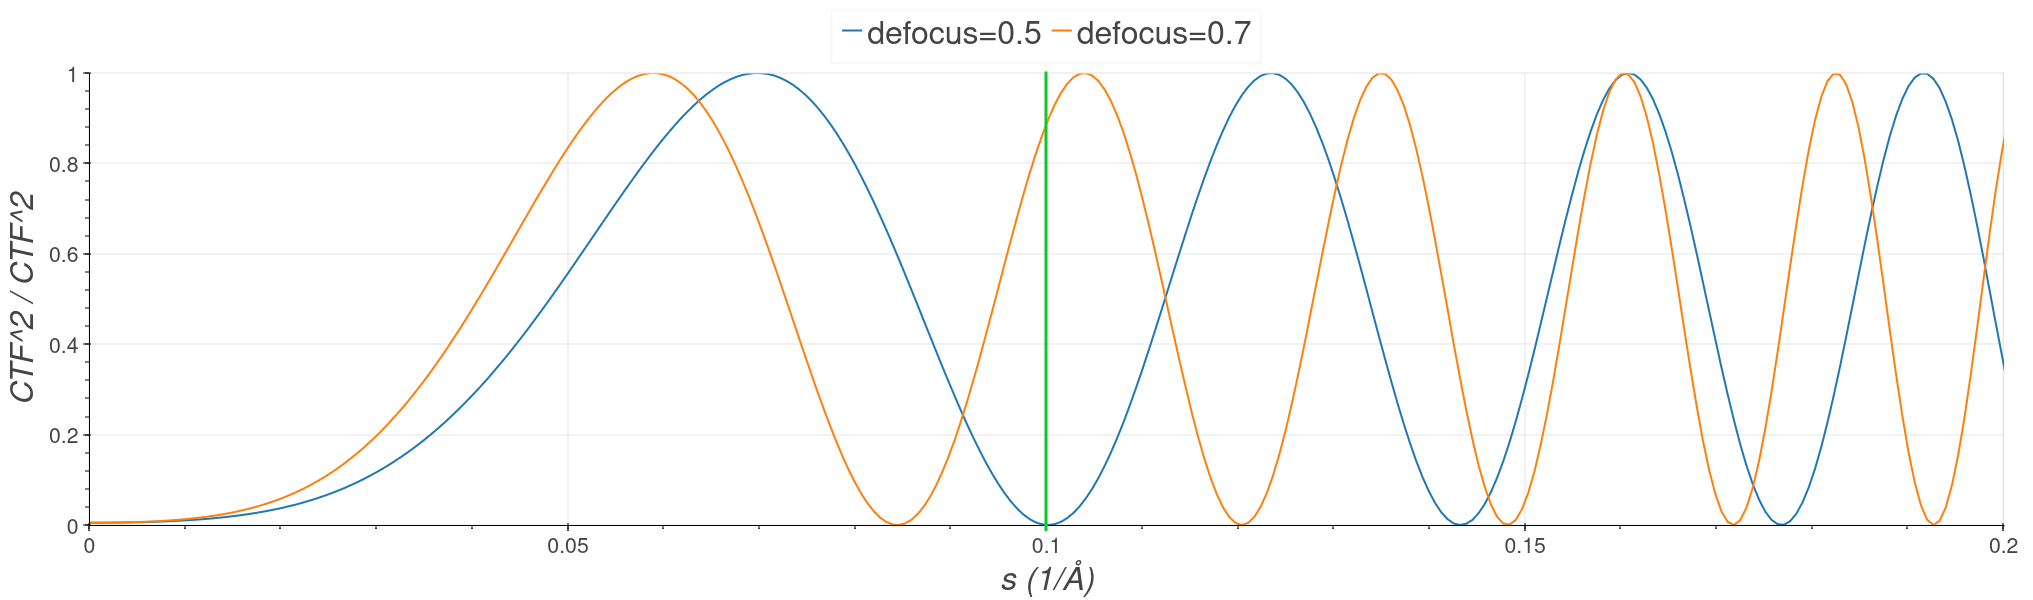
\includegraphics[width=\textwidth]{introduction/ctf_defocus_1d.png}
        \caption{1D rotational average.}
        \label{fig:em_ctf_defocus_1d}
    \end{subfigure}%

    \caption[CTF: effect of defocus]{Simulated CTF of two images at different defoci. Highlighted in green is the spatial frequency of \qty{0.1}{\angstrom^{-1}}, where there the blue line (CTF at defocus \qty{0.5}{\micro\meter}) is close to zero, whereas the orange line (CTF at defocus \qty{0.7}{\micro\meter}) is close to 1. Image generated with: \url{https://ctfsimulation.streamlit.app/}~\cite{jiangWebbasedSimulationContrast2001}.}
    % https://ctfsimulation.streamlit.app/?ctf_type=CTF%5E2&ctf_type=CTF%5E2&defocus=0.5&defocus=0.7&over_sample=6&over_sample=6&share_url=1&show_2d=1
    \label{fig:em_ctf_defocus}
\end{figure}

To ensure all spatial frequencies are sampled, a data collection must include many images collected at a range of different defoci.

Of note is that since the CTF starts at \num{0}, low spatial frequencies are always dampened; in pratical terms, this results in images where low resolution features (such as membranes and big objects) are harder to see, making it harder to distinguish objects from the noise, pick particles (see \fullref{em_particle_picking}) and do further processing.
For this reason, a certain amount of defocus is always used, unfortunately at the cost of jumbling up the high frequency information with more CTF oscillation.
Alternatively, a phase plate can be used to shift the phase of the electrons by \ang{90} and acquire images on focus (\autoref{fig:em_ctf_phase_shift}).
While phase plates are in theory the ideal solution to this problem, there are still some engineering and physical limitations that limit their use; several groups are currently working to overcome such hurdles~\cite{danevExpandingBoundariesCryoEM2017,schwartzLaserPhasePlate2019}.

\begin{figure}[ht]
    \centering
    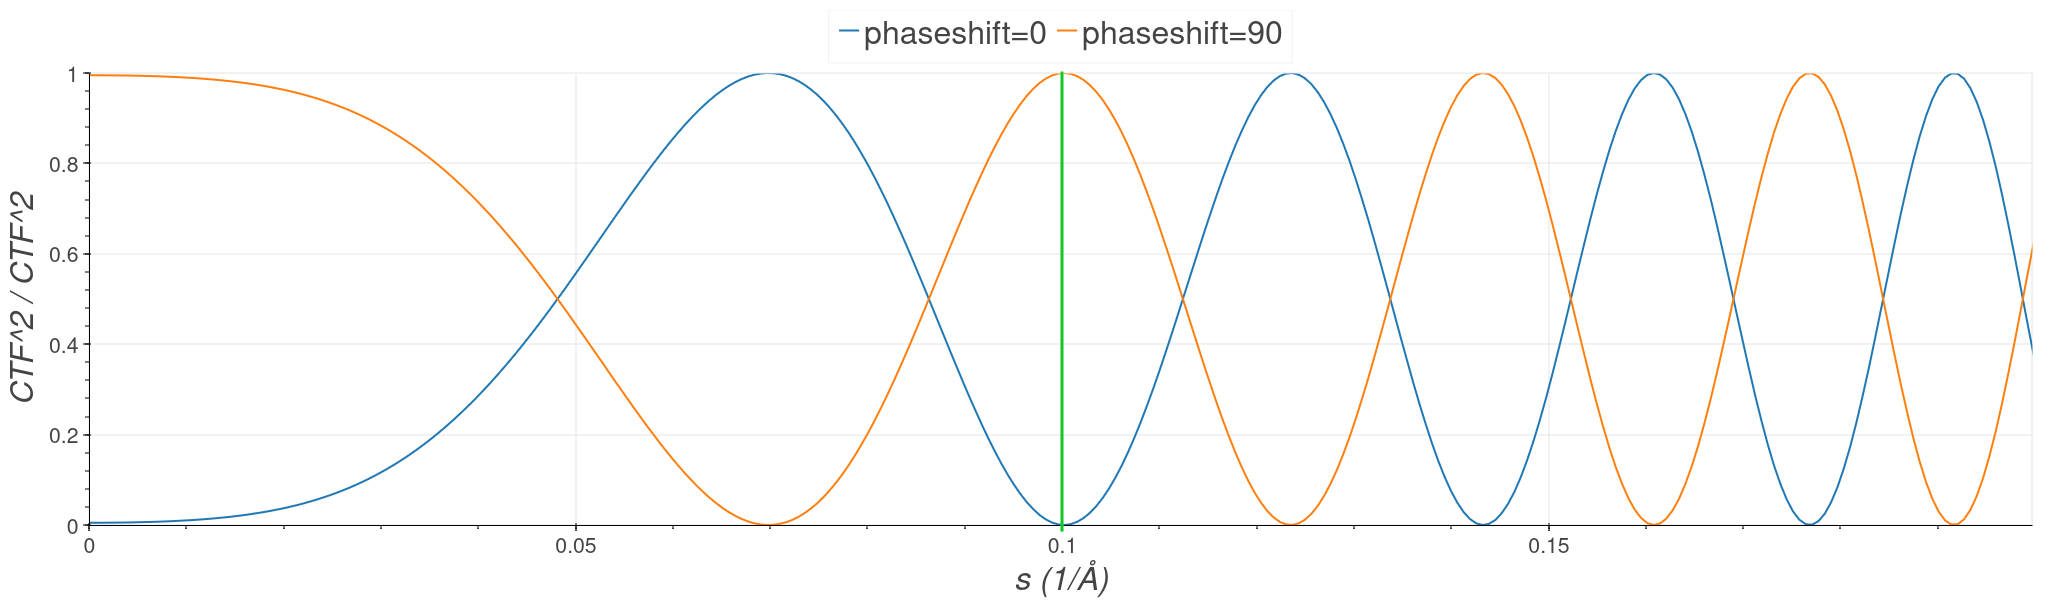
\includegraphics[width=\textwidth]{introduction/ctf_phase_shift.png}
    \caption[CTF: effect of phase shift]{Simulated CTF of two images at different phase shifts. Note how the phase-shifted CTF (orange) has a peak at spatial fequency \num{0}, boosting low-resolution features. Image generated with: \url{https://ctfsimulation.streamlit.app/}~\cite{jiangWebbasedSimulationContrast2001}.}
    % https://ctfsimulation.streamlit.app/?ctf_type=CTF%5E2&ctf_type=CTF%5E2&defocus=0.5&defocus=0.7&over_sample=6&over_sample=6&share_url=1&show_2d=1&phaseshift=0.0&phaseshift=90.0
    \label{fig:em_ctf_phase_shift}
\end{figure}

The second component of the CTF is broadly called "envelope function", a dampening effect which attenuates the signal at higher resolutions.
It depends on many factors, such as lens aberrations, limitations of the electron gun, frame alignment imprecision, etc.
This effect is visible in the PS as an attenuation of the signal at higher resolutions (\autoref{fig:em_ctf_envelope}).
Since the PS (what we actually measure) is equivalent to the $CTF^2$, the dampening is exacerbated because values closer to \num{0} become even smaller and harder to detect.
Importantly, this effect is worse at higher defocus, contributing the worse high-resolution information transfer of higher defocus images.

\begin{figure}[ht]
    \centering
    \begin{subfigure}[B]{.42\textwidth}
        \centering
        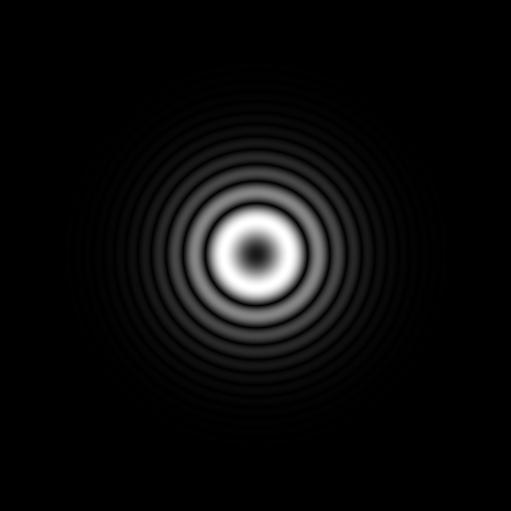
\includegraphics[width=\textwidth]{introduction/ctf_envelope_2d.png}
        \caption{2D power spectrum.}
        \label{fig:em_ctf_envelope_2d}
    \end{subfigure}%
    \hfill
    \begin{subfigure}[B]{.55\textwidth}
        \centering
        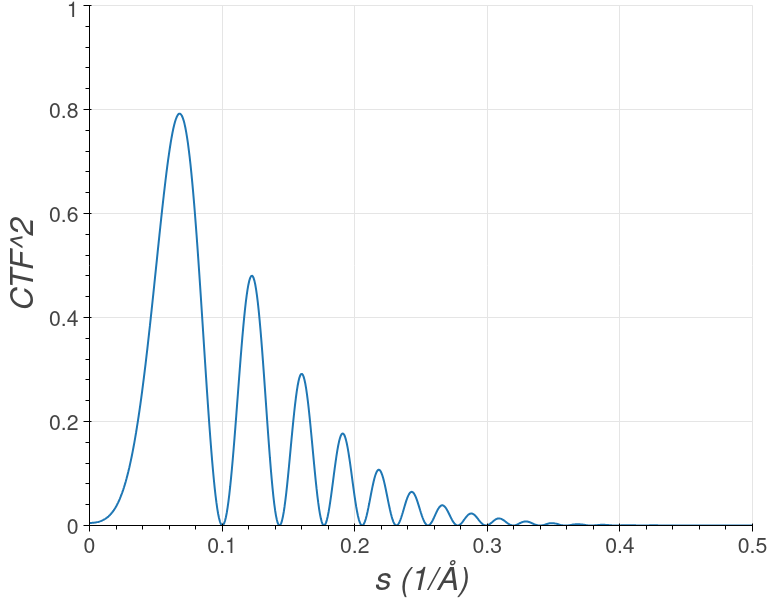
\includegraphics[width=\textwidth]{introduction/ctf_envelope_1d.png}
        \caption{1D rotational average.}
        \label{fig:em_ctf_envelope_1d}
    \end{subfigure}%
    \caption[CTF: effect of the envelope function]{Simulated CTF of an image, including some envelope function effects (such as beam convergence and energy spread). As a result, higher resolution frequencies are dampened, reducing the signal available for CTF estimation and high resolution reconstruction. Image generated with: \url{https://ctfsimulation.streamlit.app/}~\cite{jiangWebbasedSimulationContrast2001}.}
    % https://ctfsimulation.streamlit.app/?ctf_type=CTF%5E2&defocus=0.5&defocus=0.7&over_sample=3&share_url=1&show_2d=1&phaseshift=0.0&phaseshift=90.0&bfactor=10.0&alpha=0.3&dE=2.0&dI=7.0&dZ=0.1&dXY=0.1
    \label{fig:em_ctf_envelope}
\end{figure}

This signal decay, combined with the low SNR of the images, poses a resolution limit beyond which it is impossible to estimate (and therefore correct) the effect of the CTF on the image.

So far we discussed what happens to the fourier transform or PS of an image, that is in \textbf{fourier space}; in practice, the CTF has visible effects also in \textbf{real space}.
The signal becomes delocalized, blurring the image; as explained by the convolution theorem~\cite{wikipediaConvolutionTheorem2024}, this delocalization is the result of the convolution of the fourier transform of the CTF (known as Point Spread Function or PSF) with the image.
Delocalization of signal directly affects how image processing is performed; for example, particle picking should account for it by extracting bigger image patches to ensure delocalized signal can be deconvolved when CTF correcting (see \fullref{em_particle_picking}).

\subsection{Preprocessing}\label{em_preprocessing}

Before particle picking, classification, and 3D reconstruction can be performed, the collected data must undergo a few preprocessing steps.

First, each movie generated during data collection must be aligned and averaged.
In state of the art applications, this alignment is typically done not only on a full frame level, but also in a localized fashion, by aligning image patches or by describing the system with a smooth deformation field~\cite{zhengMotionCor2AnisotropicCorrection2017,punjaniCryoSPARCAlgorithmsRapid2017,tegunovRealtimeCryoelectronMicroscopy2019}.

In state of the art software, similarly to how motion correction is treated, defocus (and thus CTF) is estimated at a local level, accounting for variability in the positioning of the sample with respect to the detector.
The parameters thus obtained are later used to correct for the CTF during classification and reconstruction (see \fullref{em_classification} and \fullref{em_reconstruction}).
Modern workflows also offer the ability to later refine the deformation parameters as part of the refinement process (see \fullref{em_refinement}).

Both motion correction and CTF estimation --- as well as many other steps and techniques in image processing --- rely on the ability to quantify the similarity of two signals; this is typically done by calculating the cross-correlation (CC) of the images or signals.

\subsubsection{Cross-correlation}\label{em_cross_correlation}

The CC of two signals (such as two images) is a measure of how similar the two signals are at all possible relative shifts.
The CC function of two signals will be higher for signals that present more similar features, and have a peak at the relative shift where the signals present strongest similarity (\autoref{fig:em_cross_correlation}).
This is a useful feature for most applications, because we often care about where exactly the similarity is high (e.g. for motion correction and particle picking (see \fullref{em_particle_picking})).

\begin{figure}[ht]
    \centering
    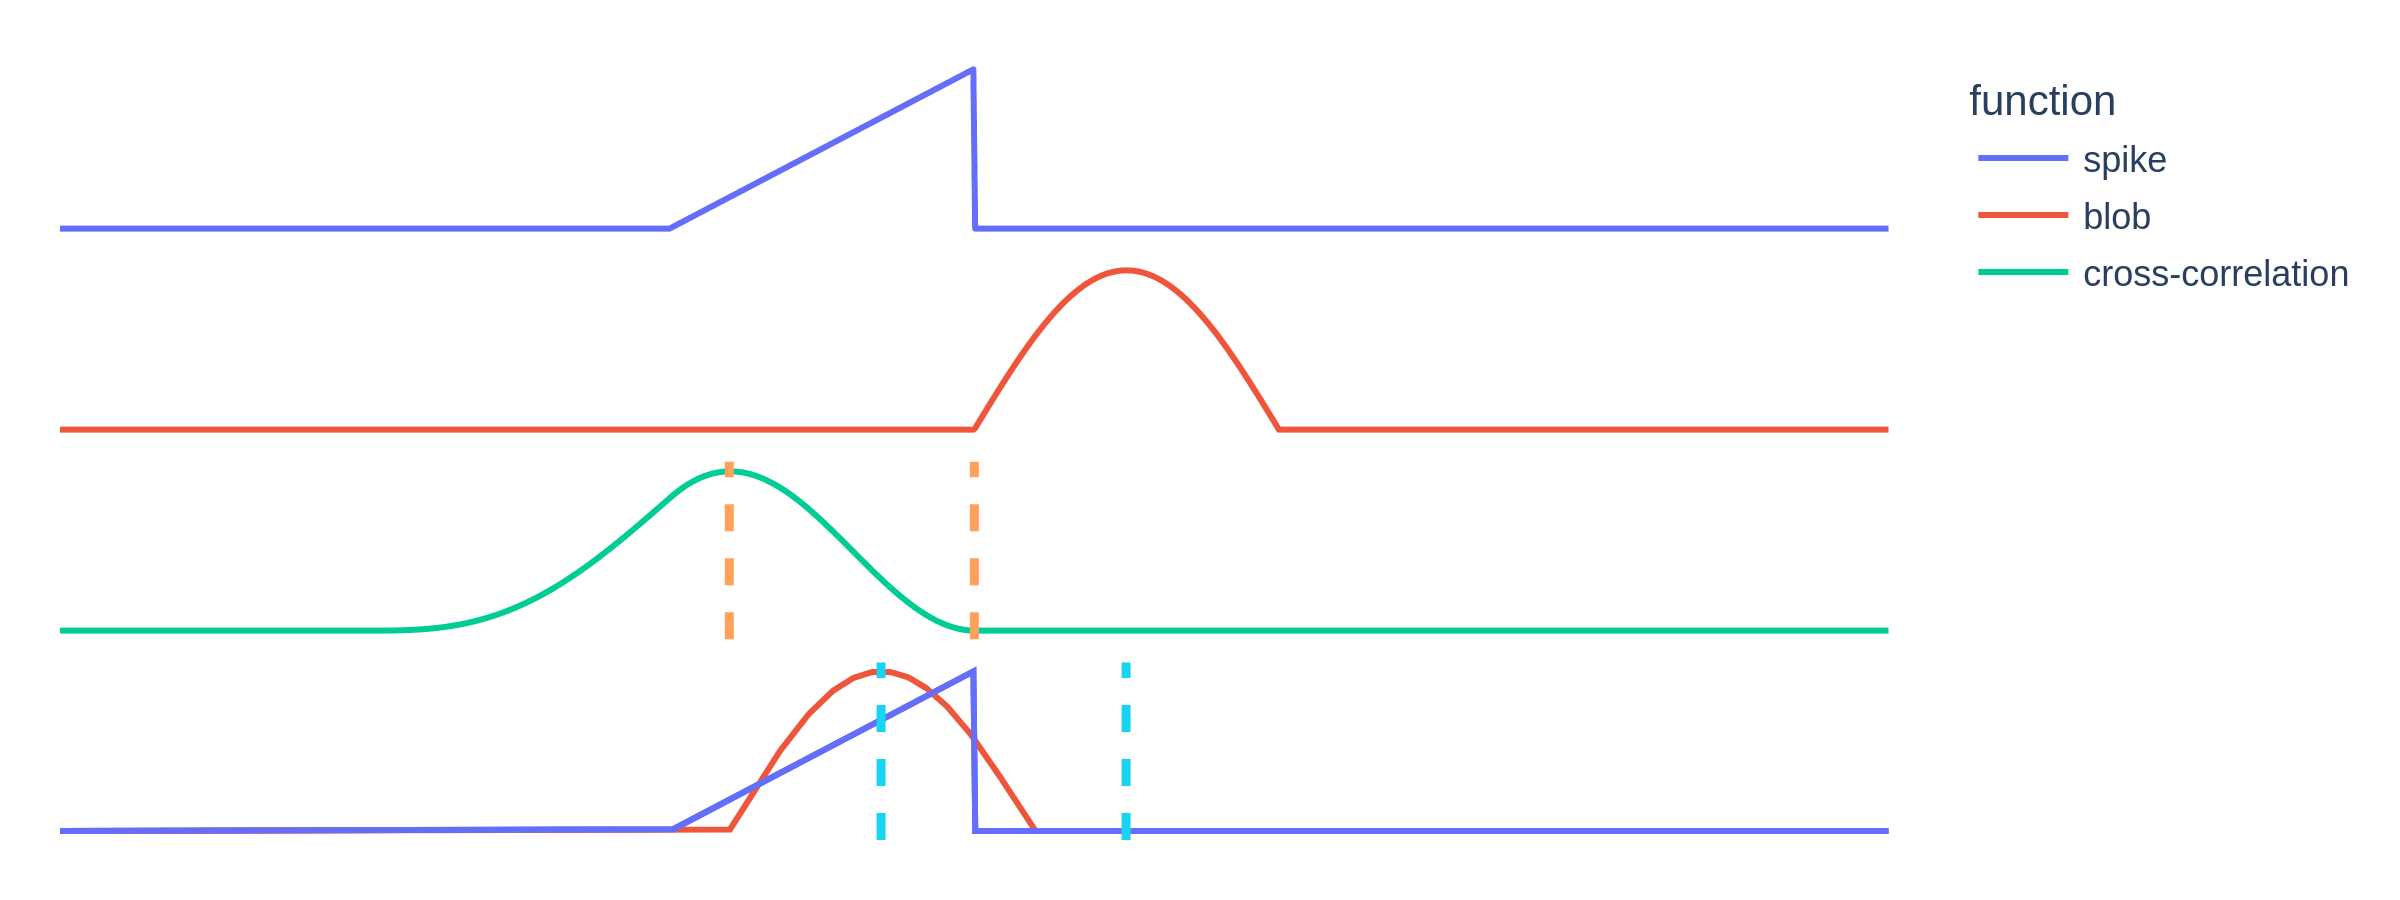
\includegraphics[width=\textwidth]{introduction/cross_correlation.png}
    \caption[Cross-correlation of 1D signals]{Cross-correlation of two 1D signals, \texttt{spike} and \texttt{blob}. The position of the peak of the resulting \texttt{cross-correlation} indicates relative shift at which \texttt{blob} presents maximal similarity with \texttt{spike}. Shifting \texttt{blob} by the same amount shows the best overlap between the two signals.}
    \label{fig:em_cross_correlation}
    % TODO: generated with cc_image.py script. Should add somehow to thesis!
\end{figure}

In the case of 2D data, calculating the cross-correlation of two images often also includes the additional step of a rotational search, to account for the different in-plane rotation of particles that would otherwise be missed by simple CC.

\subsubsection{Filtering and denoising}\label{em_filtering_and_denoising}

Due to the low SNR of cryo-EM data, even motion-corrected micrographs can can be surprisingly hard to interpret.
To enhance the contrast of biological features and better judge the quality of the data --- as well as improve the ability to distinguish particles from the background and from one another for the purposes of picking (see \fullref{em_particle_picking}) --- micrographs often undergo a round of filtering and/or denoising.

The simplest --- and most commonly used --- type of filtering is fourier masking; by reducing or zeroing the values inside a disc or annulus in fourier space, the respective spatial frequencies are dampened in the image.
In practice, this is often used to remove high-frequency components (low-pass filter), but there are also sometimes benefits to the removal of other ranges of spatial frequencies (\autoref{fig:em_filtering}).

\begin{figure}[ht]
    \centering
    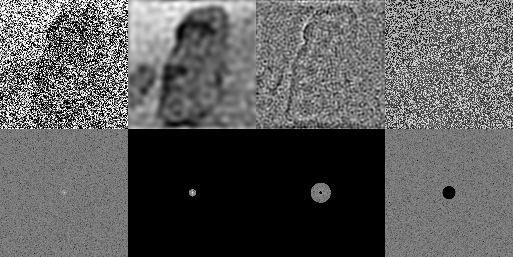
\includegraphics[width=\textwidth]{introduction/filtering.png}
    \caption[Fourier filtering]{Examples of how filtering a noisy image (top left image) with different kinds of fourier masks (bottom row) produces different results (top row). From left to right: no filtering, low-pass, band-pass, high-pass. Low-pass filtering can restore interpretability of highly noisy images. As highlighted by the difference between the low-passed (second column) and high-passed (last column) images, a very small range of low spatial frequencies is actually responsible for the majority of our perception of the general shape of an object. Noise, on the other hand, more strongly affects high resolution information.}
    \label{fig:em_filtering}
    % TODO: made with filter.py
\end{figure}

In the last few years, ML-based denoising has become standard practice, with algorithms such as noise2noise and noise2void~\cite{lehtinenNoise2NoiseLearningImage2018,krullNoise2VoidLearningDenoising2019} being implemented in several cryo-EM software suites~\cite{beplerTopazDenoiseGeneralDeep2020,tegunovRealtimeCryoelectronMicroscopy2019,buchholzCryoCAREContentAwareImage2018}.

\subsubsection{Dataset cleaning}
The dataset often contains bad images for various reasons: bad CTF estimation, too high motion, issues with autofocus, too thick or cracked ice, etc.
During preprocessing, these micrographs are usually discarded, either manually or by using batch automated tools which estimate the data quality.

Once the data is clean, motion corrected and CTF-estimated, the particles of interest can be picked for further processing.

\subsection{Particle picking}\label{em_particle_picking}
In order to reconstruct the 3D map of particles of interest, one first needs to locate them on the micrograph.
This procedure is called particle picking, and can be performed with varying levels of automation, and using several different techniques.
The most commonly used are variations of: manual picking, template matching, and machine learning (ML) tools.

Manual picking is generally more intuitive and can be very precise, but is also tedious and time-consuming.
Data may also be too noisy for humans to distinguish particles from one another and from the background, leading to missed particles or wrong picks.
To aid with manual picking, preprocessed micrographs are often filtered and denoised to improve the contrast (see \fullref{em_filtering_and_denoising}).

To improve the picking speed and precision, template matching is often used to automate searching for a recognizable object.
This picking method requires a template, a small image of a 2D projection of the object of interest.
This can be obtained in a few ways: synthetically (by using a generated shape), by projecting a known map or model from previous work, or by using the results of a first round of 2D classification (see \fullref{em_classification}) from a preliminary manual picking.
While the exact details of the algorithm may vary, at its core template matching relies on calculating the CC (see \fullref{em_cross_correlation}) function between the template and the micrographs in order to locate putative particles positions in the whole dataset.

TODO: figure with template and picks on the micrograph?

More recently, template matching is often being replaced with machine learning, which serves a similar purpose but can have a more nuanced understanding of surrounding context which helps reduce the false negatives and positives that are intrinsically present with template matching of noisy data.

There are also "structured" variants of all these picking methods, where some existing geometric and structural knowledge about the system is used to inform the picking in some way.
For example, filament picking is quite commonly used due to how widespread helical assemblies are in biology; it can be done manually~\cite{scheresRELIONImplementationBayesian2012,heHelicalReconstructionRELION2017}, with template-based methods~\cite{punjaniCryoSPARCAlgorithmsRapid2017}, and using ML~\cite{wagnerSPHIREcrYOLOFastAccurate2019,wagnerEvolutionSPHIREcrYOLOParticle2020}.

Regardless of the picking method, it is important to ensure that the target object is represented with projections from many different orientations; this will be crucial to properly reconstruct a 3D map of the object (see \fullref{em_reconstruction}).

\subsection{2D classification}\label{em_classification}

Even with the best data and most advanced methods, picked particles typically contain a variety of several different objects, conformations, and spurious background picks; before moving on to reconstruction, useful particles need to be separated from the chaff.
To do so, particles are separated into groups based on similarity, in a process called 2D classification.

Once again, some form of cross-correlation (see \fullref{em_cross_correlation}) is involved in the process, since the goal is to cluster together similar particles and separate different ones.
The algorithm is typically iterative: after generating a initial classes by averaging random particles, particle poses are progressively refined to find the best CC score.
Based on this score, each particle is assigned to a class (or a score for each class, in probabilistic models~\cite{scheresRELIONImplementationBayesian2012}), and for each class a class average is computed, combining the signal from all the particles belonging to that class. The more poses are refined, the more the signal that's shared by similar particles is boosted, improving the SRN of the class average.
Class averages are used to calculate the CC at each iteration, and used at the end of the process to inspect the dataset and select only the useful particles (\autoref{fig:em_classification}).

\begin{figure}[ht]
    \centering
    \includegraphics[width=.5\textwidth]{example-image.png}
    \caption{TODO: screenshot of classification from cryosparc}
    \label{fig:em_classification}
\end{figure}

With this information, particle classes can be split into groups for further processing or discarded.
This is typically done manually by inspecting class averages and assigning each class to a group, depending on the goals of the project and the following processing steps.
For a uniform purified dataset, classification might only serve the purpose of discarding spurious picks.
For trickier samples (protein complexes, high conformational variability, non-uniform orientation distribution, "shotgun" cryo-EM~\cite{suBuildRetrieveMethodology2021,kyrilisIntegrativeBiologyNative2019}), multiple groupings and several rounds of classification may be necessary to isolate each relevant state.

Once reasonably sure that each group contains only particles representing projections of different orientations of copies of the same object, the 3D map of this object can be reconstructed.

\subsection{3D reconstruction}\label{em_reconstruction}

3D reconstruction is the process by which a volumetric map of an object can be reconstructed from 2D projections.
This is possible thanks to the central slice theorem~\cite{wikipediaProjectionsliceTheorem2023}, which provides a bidirectional mathematical relationship between a volume and its projections.

The theorem states that the fourier transform of the 2D projection of a volume at a certain orientation, is equal to the central slice through the fourier transform of the volume at the orientation perpendicular to the projection (\autoref{fig:em_central_slice}, panel A).

It's worth noting that the algorithms used by reconstruction software, while based on this principle, are often in practice not based on fourier-domain reconstruction, but use different methods such as weighted back-projection or iterative approaches like SART and SIRT~\cite{andersenSimultaneousAlgebraicReconstruction1984,agulleiroFastTomographicReconstruction2011,wikipediaTomographicReconstruction2024}.

\begin{figure}[ht]
    \centering
    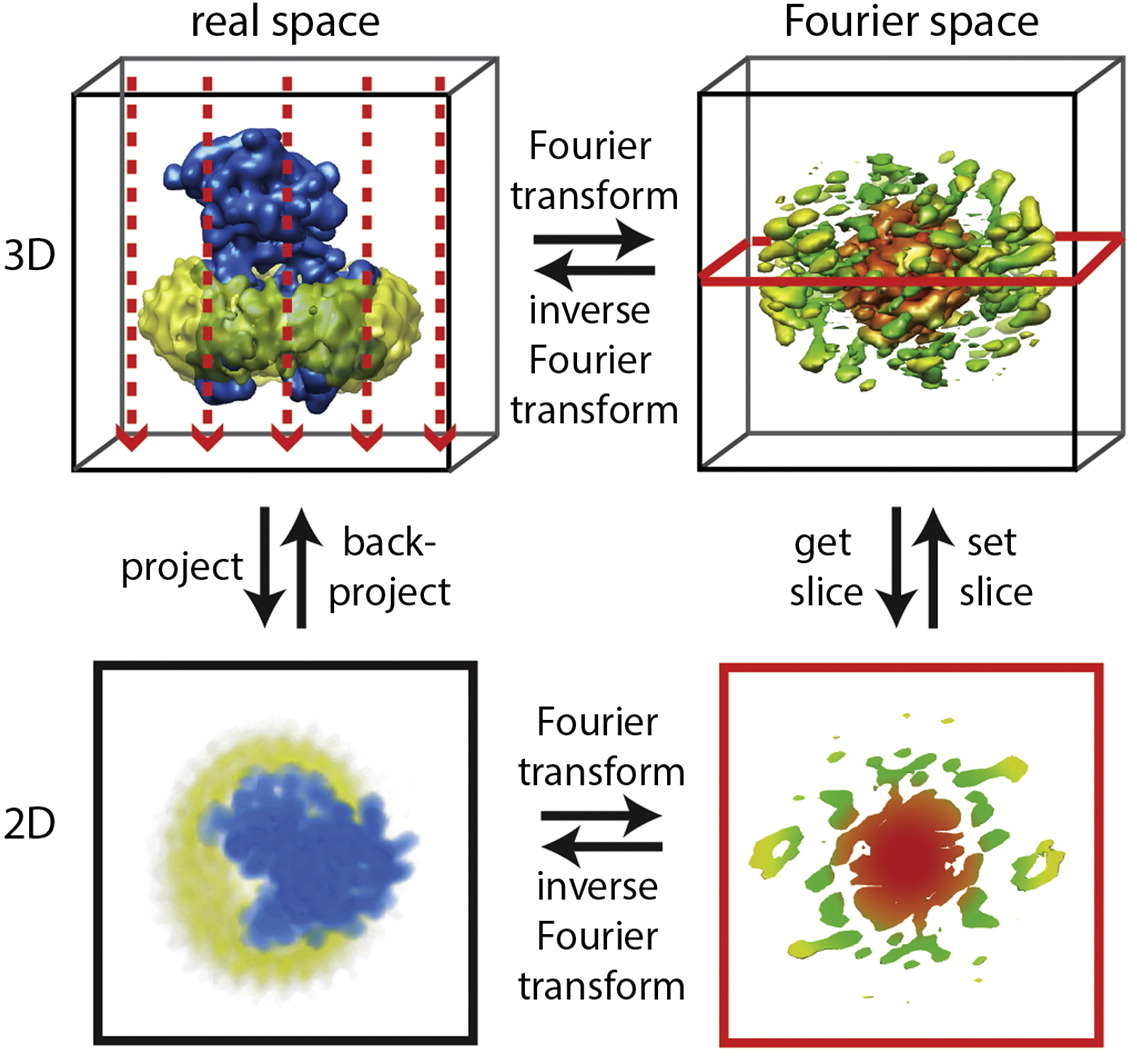
\includegraphics[width=.7\textwidth]{introduction/central_slice_theorem.png}
    \caption[Central slice theorem]{Showcase of how the central slice theorem is used for 3D reconstruction in cryo-EM. \textbf{A.} A 2D projection of a 3D volume in real space at a certain orientation is equivalent to the 2D slice perpendicular to that orientation in fourier space. \textbf{B.} \textbf{C.} \textbf{D.} \textbf{E.}. Figure adapted from \citet{nogalesCryoEMUniqueTool2015}.}
    \label{fig:em_central_slice}
\end{figure}

In the case of SPA, the central slice theorem allows us to combine the projection of many different particles, under the assumption that they come from near-identical copies of the same object.

It is crucial in this process that as many different orientations as possible are represented in the dataset.
This is because, in order to have an isotropically well-resolved reconstruction, we need to fill the 3D fourier space as much as possible with differently oriented central slices.

Similarly to 2D classification, 3D reconstruction is an iterative process where each particle is correlated to templates to find the best match.
This time, however, the templates are obtained by projecting a 3D model at different orientations, in a process called projection matching (\autoref{fig:em_projection_matching}).
Instead of assigning classes, projection matching refines the relative (3D) orientations of each particle relative to the original 3D object.
The 3D model is initally either derived from previous work, or generated \textit{ab initio} from the particles themselves.
During each iteration, particles' FTs are used to fill a 3D FT according to central slice theorem, which allows to generate a new 3D model.
The assigned orientations are progressively refined in order to improve the model resolution.
Once there is no longer significant improvement (see \fullref{em_fsc}), the process stops, and the final 3D map is generated.

\begin{figure}[ht]
    \centering
    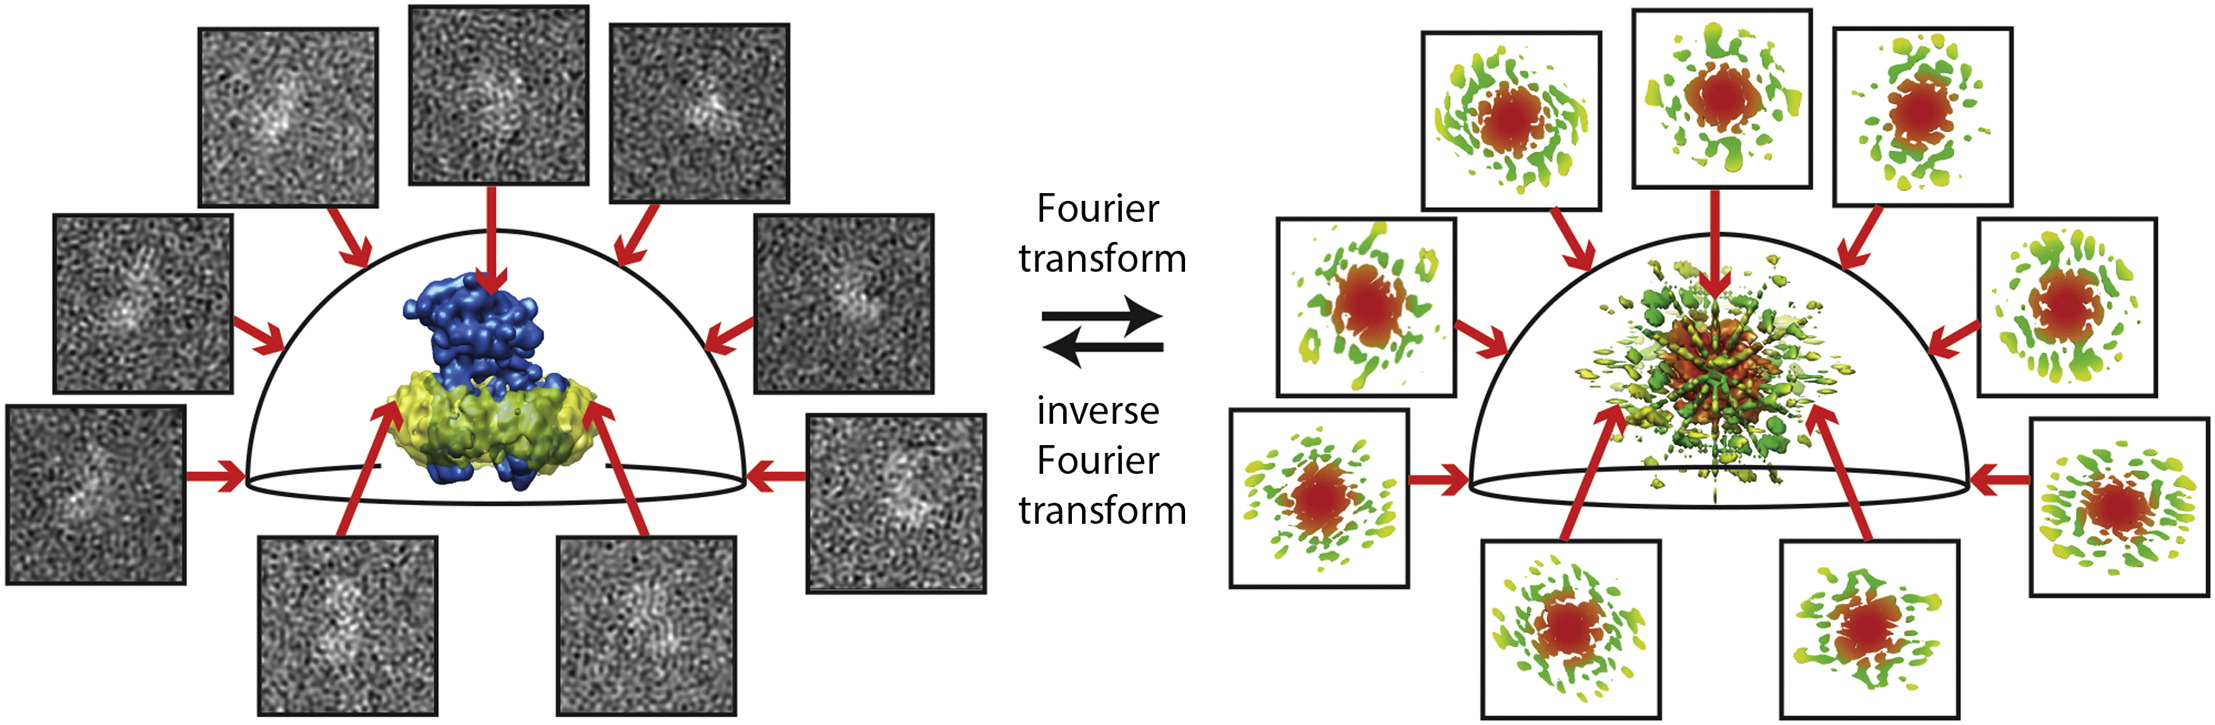
\includegraphics[width=\textwidth]{introduction/projection_matching.png}
    \caption[Projection matching]{Projection matching in cryo-EM. Particle picks are assigned progressively better orientations that most closely match synthetic 2D projections generated from the current 3D model. By inserting the FT of each particle at the assigned orientation into the 3D fourier space, and then doing the inverse fourier transform to go back to real space, a new updated model is generated. Figure adapted from \citet{nogalesCryoEMUniqueTool2015}.}
    \label{fig:em_projection_matching}
\end{figure}

In some cases, it might be useful to go one step further and do 3D classification; this is essentially the same procedure, but using multiple 3D models at the same time to not only assign orientations, but also split particles into different classes.
This may be useful --- especially combined with some kind of mask to isolate areas of interest --- in cases where 2D classification was unable to separate out very similar objects.

When classification is too categorical to capture nuanced systems (such as heterogeneous conformational ensembles), other kinds of procedures able to capture more variability may be used, such as principal component analysis (PCA)~\cite{castano-diezDynamoFlexibleUserfriendly2012,punjani3DVariabilityAnalysis2021}, multibody refinement~\cite{nakaneMultibodyRefinementCryoEM2021}, 3D flexible refinement~\cite{punjani3DFlexibleRefinement2022}, etc.

\subsubsection{FSC and gold standard}\label{em_fsc}
For most procedures that attempt to refine parameters in order to improve a 3D classification or reconstruction, a method is needed to estimate the quality (resolution) of the current model.

The established approach is called \textbf{gold sandard} and relies on calculating the fourier shell correlation (FSC) of two independent halves of the data.
At the cost of halving the amount of data we can use at once to make a map, we gain the ability to estimate how trustworthy our recostruction is.

At the beginning of the process, the dataset (which in the case of 3D reconstruction is the ensemble of picked particles) is randomly split in two halves.
At each iteration of the refinement, each half is used to generate an independent 3D reconstruction.
The fourier transforms of the two maps are then cross-correlated as a function of spatial frequency, giving a plot such as the one in \autoref{fig:em_fsc}.
A high correlation between fourier shell at the same spatial frequency indicates a high degree of reproducibility of those frequency components: that is, up to that resolution, the map can be trusted.
The threshold typically used to formally determine the "resolution of the map" is \num{0.143}, for both mathematical and historical reasons related to the interpretability of X-ray crystallography maps~\cite{rosenthalOptimalDeterminationParticle2003}.

\begin{figure}[ht]
    \centering
    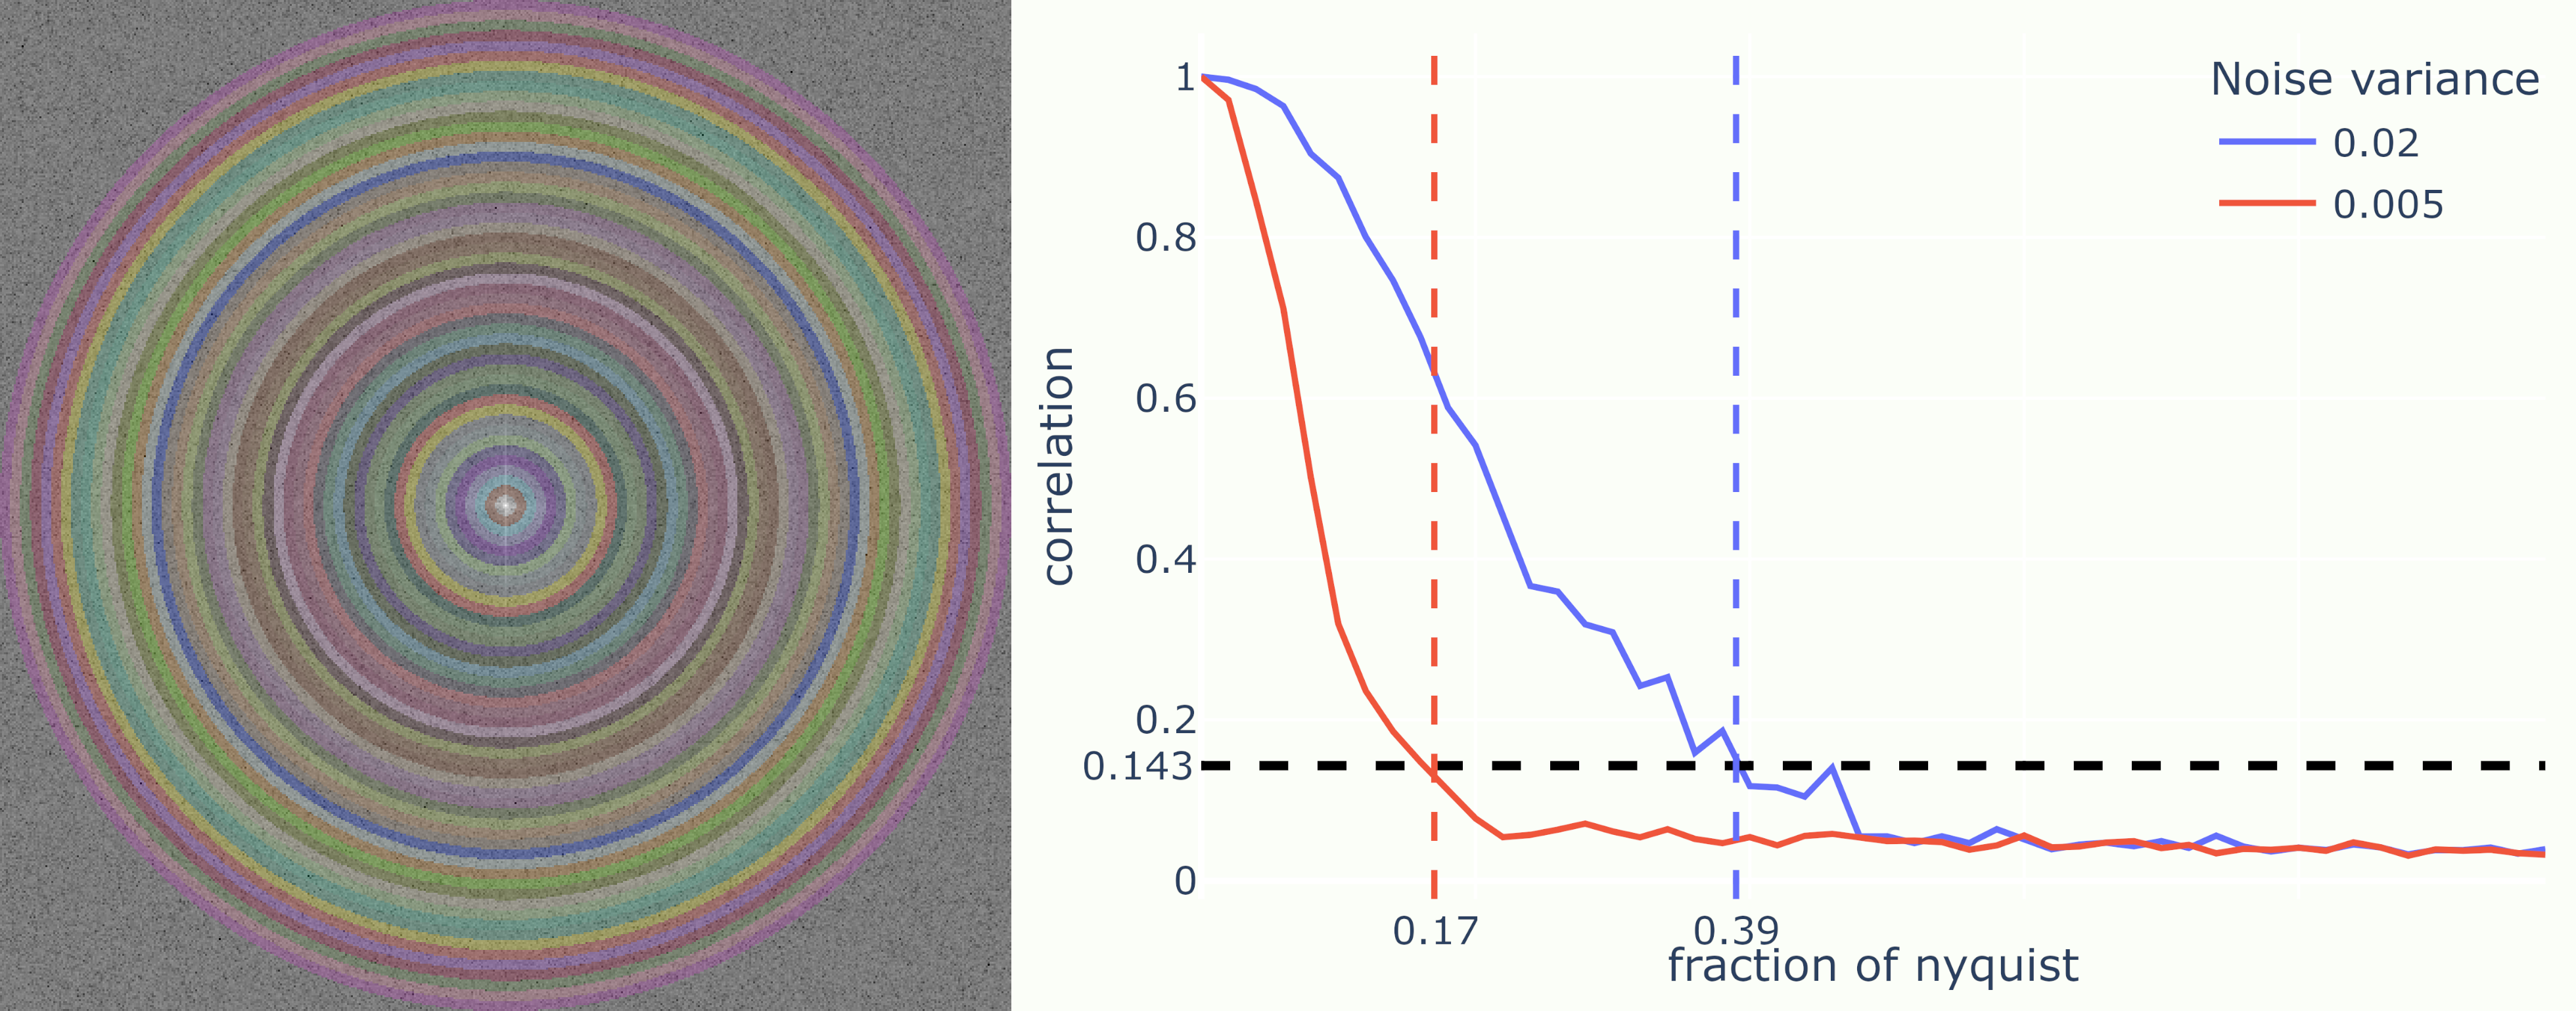
\includegraphics[width=\textwidth]{introduction/fsc.png}
    \caption[Fourier shell correlation]{Showcase of a 2D version of fourier shell correlation. Gaussian noise was applied to two identical images, which were then compared by gradually cross-correlating concentric shells (left). The resulting plot (right) is a measure of the similarity as a function of spatial frequency. As spatial frequency increases, noise becomes dominant, degrading correlation and thus the trustworthiness of the data. The threshold of \num{0.143} is used to determine the final resolution, which is higher for the less noisy image.}
    \label{fig:em_fsc}
    % TODO: made with script fsc.py
\end{figure}

\subsubsection{Map post-processing}
Reconstructed maps are normally post-processed to improve interpretability and usability in model building procedures.

Different types of masking, filtering, and denoising can be applied, depending on the downstream steps.

TODO: feels like I should expand, but it's also not very important here. Sharpening?

\subsection{Refinement}\label{em_refinement}
Once a 3D model is obtained, several state of the art software pipelines offer the ability to refine previously-defined parameters, using the estimated resolution of the 3D reconstruction validate the improvements.
The parameters that can be refined range from particle positions and orientations, to CTF estimation and motion correction, to more complex artifact-inducing factors such as lens aberrations and Ewald sphere curvature~\cite{tegunovMultiparticleCryoEMRefinement2021,punjaniCryoSPARCAlgorithmsRapid2017}.

The implementation details of refinement procedures are often quite different between software, but are generally based on an iterative process where parameters are adjusted on a per-particle basis, and a new 3D reconstruction is generated and validated via FSC to estimate the effects of the correction applied.

These procedures can have dramatic effects on the final resolution of a map, especially when pushing for near-atomic resolution where small aberrations and artifacts can have significant effects on the achievable resolution.

\subsection{Model building}

If a map reaches high enough resolution, it is possible to build an atomic model based on the volume density.
This process is called model building, and is typically done with a mix of manual and automated tools.

Models are build by placing aminoacids (or other structural components) so that their electron occupancy matches the density map obtained from 3D reconstruction.
Some recent tools manage to fully automate this process for maps of high enough resolution, even without knowing the protein's sequence~\cite{jamaliAutomatedModelBuilding2024}.

\subsection{Pros and Cons}

TODO: I don't love this section. Need some rewording/restructuring.

SPA offers some advantages and disadvantages compared to other popular techniques, making it more suitable for certain applications.

Compared to X-ray crystallography, SPA sample preparation is a strong selling point: it can be much faster and simpler, not requiring crystallization and needing small quantities of sample, and being less sensitive to contamination.
Thanks to the fast vitrification, SPA is also better for studying the sample at near-native state, and for capturing rare or dynamic states (though the analysis in these cases becomes trickier).
However, due to the unknown particle orientations and low SNR, SPA data analysis is trickier and more error-prone, especially for small particles (\lesssim\qty{100}{\kilo\dalton}).

Bigger particles or complexes are usually better handled by cryo-EM: with increasing size, crystallization gets more difficult, and NMR spectra become harder to interpret to extract complete structural information.
On the other hand, NMR takes the near-native crown, being able to collect data on a sample directly in solution, providing information about dynamics and interactions.

However, near-native is often not enough: all these techniques rely on drawing information about an ensemble of molecules, typically with a purified sample prepared \textit{in vitro}.
Often, macromolecular systems can only be fully understood by accounting for their biological context, which is partly or fully lost in the expression and purification process.
When studying biological systems that form larger mesoscale and dynamic complexes, having a three-dimensional understanding of invididual events within their context becomes paramount.

A method that promises to solve these problems is cryo-electron tomography: a technique that can look not only at purified samples, but at entire organisms, \textit{in situ} and near-native conditions, with the ability to reach high resolutions via subtomogram averaging, while retaining contextual information and providing a 3D view into single events.


\section[Cryo-ET and STA]{Cryo-electron tomography and subtomogram averaging}

Tomographic reconstruction is not a recent invention: the first appearance goes back more than a century~\cite{jDeterminationFunctionsTheir1917}; its successful application to cryo-EM, however, is only a recent development closely linked to the resolution revolution, which allowed to finally overcome the biggest overarching limitation of cryo-ET --- poor signal-to-noise ratio --- enough to reach sub-nanometer resolutions~\cite{lucicCryoelectronTomographyChallenge2013,turkPromiseChallengesCryoelectron2020}.

At its core, cryo-ET is just cryo-EM with extra steps; they share much of the theory, hardware and software.
The key difference is that, where single particle cryo-EM uses projections from different \textit{copies} of the same object to reconstruct a 3D map, cryo-ET images the same location from multiple orientations in order to reconstruct a 3D map from multiple projections of the \textit{same} object.
This section describes the theory of cryo-ET, how it deviates from SPA, and the current state of the art with its limitations and upcoming developments.

\subsection{Sample preparation}
As with SPA, vitrification remains the key step of sample preparation for cryo-ET.
Due to the intrinsically worse SNR due to the lower electron dose used during data collection (see \fullref{et_data_collection}), cryo-ET sample preparation requires extra care to reduce any possible source of additional noise.

One such source is the thickness of the sample; unfortunately, this is often antithetical to samples such as entire cells or organelles, where cryo-ET \textit{in situ} benefits really shine.
Initially, this problem was tackled by either prepararing simpler model systems \textit{in vitro} --- moving partly away from the native state --- or by cutting thin slices from a thicker sample via cryo-ultramicrotomy~\cite{peaseElectronMicroscopyUltramicrotomy1981}.
In recent years, focused ion beam (FIB) milling, a technique already well established in material sciences, has found widespread use in cryo-ET sample preparation, allowing to slice thin lamellae from a vitrified sample without incurring in the shear and surface deformations of cryo-ultramicrotomy~\cite{markoFocusedionbeamThinningFrozenhydrated2007}.

\subsubsection{FIB milling}
FIB milling typically makes use of a Gallium ion beam --- or, more recently, Xenon plasma --- to ablate a sample
thick samples can be thinned to below \qty{150}{\nano\meter}.
Preparing lamellae via FIB milling is becoming standard procedure in cryo-ET, but is still far from being consistently reproducible and automatable.

\begin{figure}[ht]
    \centering
    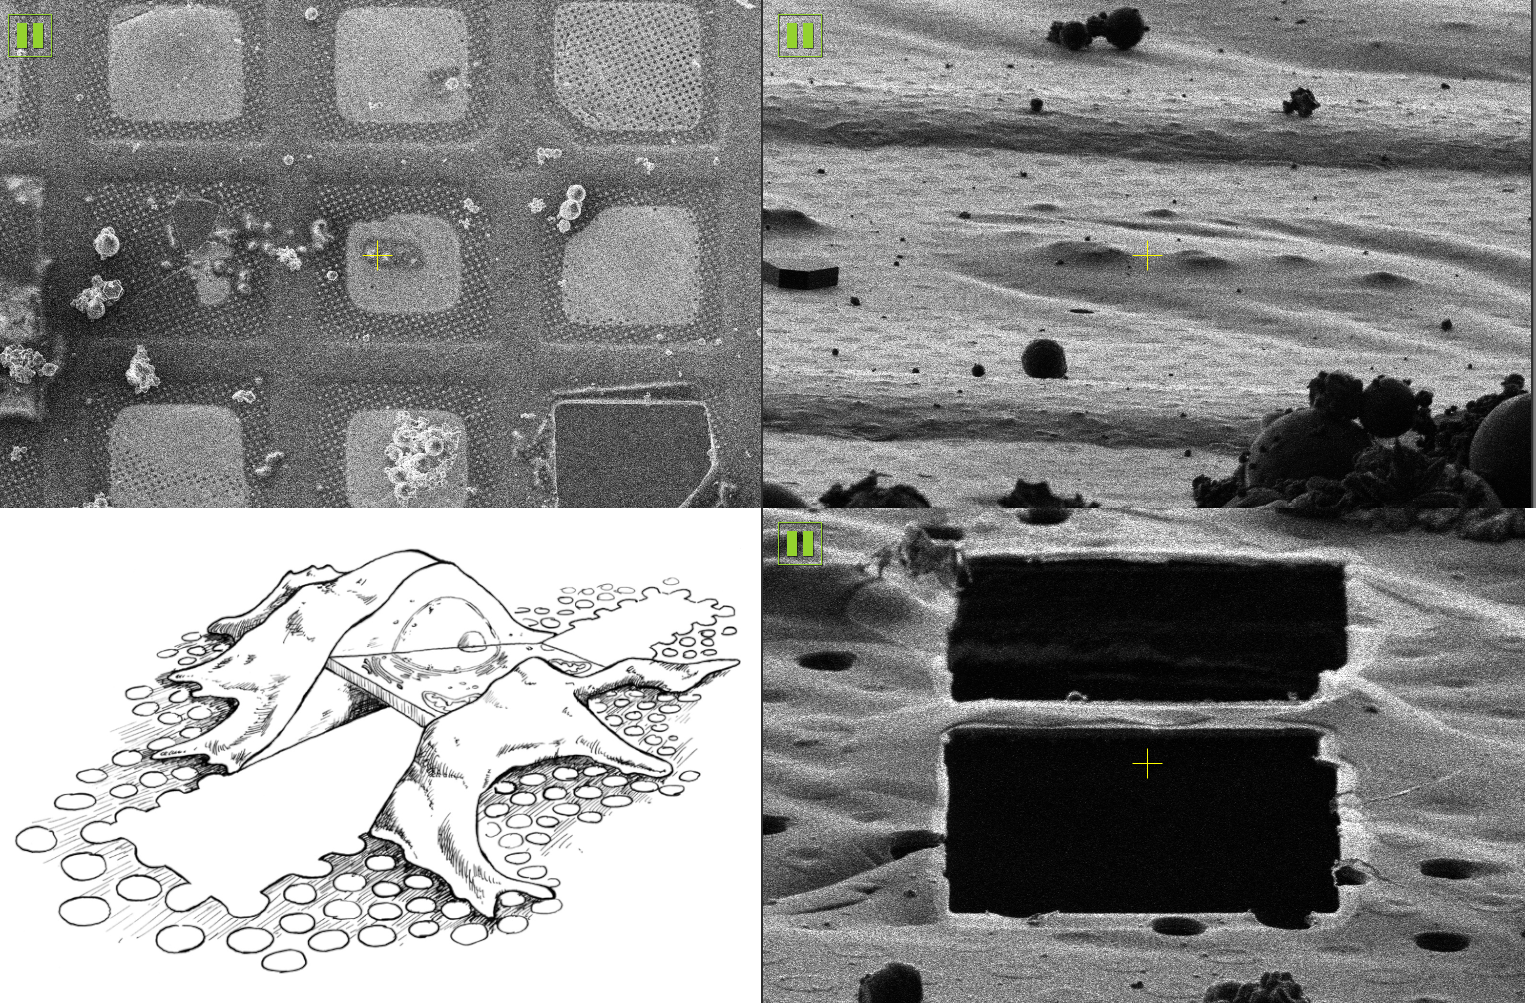
\includegraphics[width=\textwidth]{introduction/fib.png}
    \caption[FIB milling]{Microscope snapshots from FIB milling procedure on \textit{Deinococcus radiodurans}. A cluster of cells, visible as a bump on the SEM, is selected from the grid (top left). From a shallow angle of around \ang{15} from the grid (top right) the FIB is used to ablate material above and below the area of interest. This leaves a thin lamellae suitable for cryo-ET (bottom). Milled cell drawing (bottom left) taken from ~\citet{villaOpeningWindowsCell2013}.}
    \label{fig:et_fib_milling}
\end{figure}

\subsubsection{Fiducials}\label{fiducials}
During data collection, despite vitrification, samples undergo different kinds of deformations.
Moreover, due to the intrinsic imprecision of controlling the hardware of the microscope, there will always be some shift and angle mismatch between different tilts during a tilt series collection (see \fullref{et_data_collection}).

To help with correcting these errors, it is often useful to add to the same some fiducials: small high-contrast, round objects (typically gold beads) that can later be used to estimate sample shift, rotation, and deformations (see \fullref{et_tilt_series_alignment}).

\subsection{Data collection}\label{et_data_collection}
In order to acquire a sequence of images at different tilts (termed \textbf{tilt series}) for tomographic reconstruction, the same area of the sample needs to be imaged at a range of different angles.
This requires longer and more sophisticated routines compared to SPA, since for each tilt angle the sample stage must be moved, the eucentric height reestablished, the lens refocused.

Due to the multiple exposures, in order to preserve the specimen from radiation damage the electron duse must be fractionated to much lower than typical in SPA, but still high enough to capture enough signal to allow motion correction~\cite{mcewenRelevanceDosefractionationTomography1995}.

Each subsequent exposure further damages the sample, which degrades the high resolution information first.
This, in combination with the fact that in cryo-ET the electron beam has to traverse a thicker sample at high tilts --- leading to worse SNR --- created the need for optimized collection schemes.
The most commonly used nowadays is the Hagen (or dose-symmetric)  scheme~\cite{hagenImplementationCryoelectronTomography2017}: it collects the first image at \ang{0} tilt, and then alternates between negative and positive tilts until it reaches the maximum tilt.
This minimizes the radiation damage when SNR is best, allowing to capture high resolution information at its prime, before it is degraded.

Due to the geometry of the sample and its support within the microscope, there is a limit to how high an angle can be reached when tilting the sample.
This angle is typically around \ang{60}-\ang{70}, beyond which either the sample grid comes into view, or the sample becomes too thick for imaging at such low doses.
This will result in a \textbf{missing wedge} of information during tomographic reconstruction (see \fullref{et_tomo_reconstruction}).

Conventional wisdom sets the interval between subsequent tilts at around \ang{3} to ensure enough fourier space filling while limiting radiation damage, though depending on the application --- especially where certain spatial frequencies are considered important or over-represented in the sample --- it might be worth considering smaller, wider, or non-linear increments~\cite{copeCryoElectronTomographyStructural2011}.

\subsection{Preprocessing}
Cryo-ET data undergoes similar preprocessing steps as SPA data (see \fullref{em_preprocessing}), albeit with less precision due to the low electron dose.

While at this point single particle data is ready for particle picking and other downstream work, cryo-ET data must still undergo tomographic reconstruction in order to obtain the 3D volumetric reconstruction of the sample.

To do so, tilt series alignment parameters must first be estimated in order to correct for equipment imprecision and sample deformations, and then used the 3D volume reconstruction.

\subsubsection{Tilt series alignment}\label{et_tilt_series_alignment}
The most basic alignment procedures require at least full-frame aligment; similar to motion correction, tilt images are rotated and shifted in order to maximize their CC score.
Where fiducials are present (see \fullref{fiducials}), these can be treated as static points within the sample and used instead as anchors to mathematically estimate the geometric transformation between different tilts~\cite{nicastroMolecularArchitectureAxonemes2006,heumannClusteringVarianceMaps2011,castano-diezDynamoCatalogueGeometrical2017}.

In state of the art software, alignment procedures (with or without fiducials) can also account for spatio-temporal deformations of the sample, either already during tilt series alignment~\cite{zhengAreTomoIntegratedSoftware2022}, or later during refinement~\cite{tegunovMultiparticleCryoEMRefinement2021,burtImageProcessingPipeline2024,galaz-montoyaSingleParticleTomography2015,chenCompleteDataProcessing2019} (see \fullref{et_refinement}).

\subsubsection{Tomogram Reconstruction}\label{et_tomo_reconstruction}
Similarly to how 3D reconstructions are obtained from 2D particles in SPA based on the central slice theorem (see \fullref{em_reconstruction}), the aligned tilt series can be used to reconstruct the full tomogram.
Depending on the software suite and workflow, full tomogram reconstructions may be used only for template matching (see \fullref{et_particle_picking}) and segmentation purposes, or also to extract subtomograms at small pixel sizes for subtromogram averaging (see \fullref{et_sta}).

Differently from SPA, cryo-ET has the advantage of knowing the 3D positioning of features in the tomogram.
This allows to bring defocus estimation and CTF correction to the next level: not only is CTF locally estimated depending on the in-plane position of features, but also accounting for the defocus difference between the top and bottom of the sample.
While this idea was around for a long time, only in recent years tools were developed that can run in reasonable time and significantly improve the final resolution~\cite{turonovaEfficient3DCTFCorrection2017,tegunovRealtimeCryoelectronMicroscopy2019}. 
Depending on the software, 3D-CTF might be estimated and corrected at different levels (tilt image, full tomogram or subtomogram), and may be able to be refined during refinement (see \fullref{et_refinement}).

Due to the limited range of tilt angles collected in typical cryo-ET workflows, not all views of the sample are represented; when reconstructing the 3D FT of the sample, this is clearly visible in in fourier space as a wedge of missing information (\autoref{fig:et_missing_wedge}).
The missing wedge introduces several problems in downstream processing: it blurs the tomogram in the Z direction, it biases subtomogram alignment, and it leads to anisotropic resolution for objects with preferential orientation.

If fiducials (or other high-contrast objects of no real interest) are present in the sample, it is often useful to mask them during reconstruction, in order to avoid the high-contrast artifactual streaks caused by the missing wedge, which can impair the interpretability of the tomogram~\cite{tegunovRealtimeCryoelectronMicroscopy2019,burtTeamtomoFidder2024}.

\begin{figure}[ht]
    \centering
    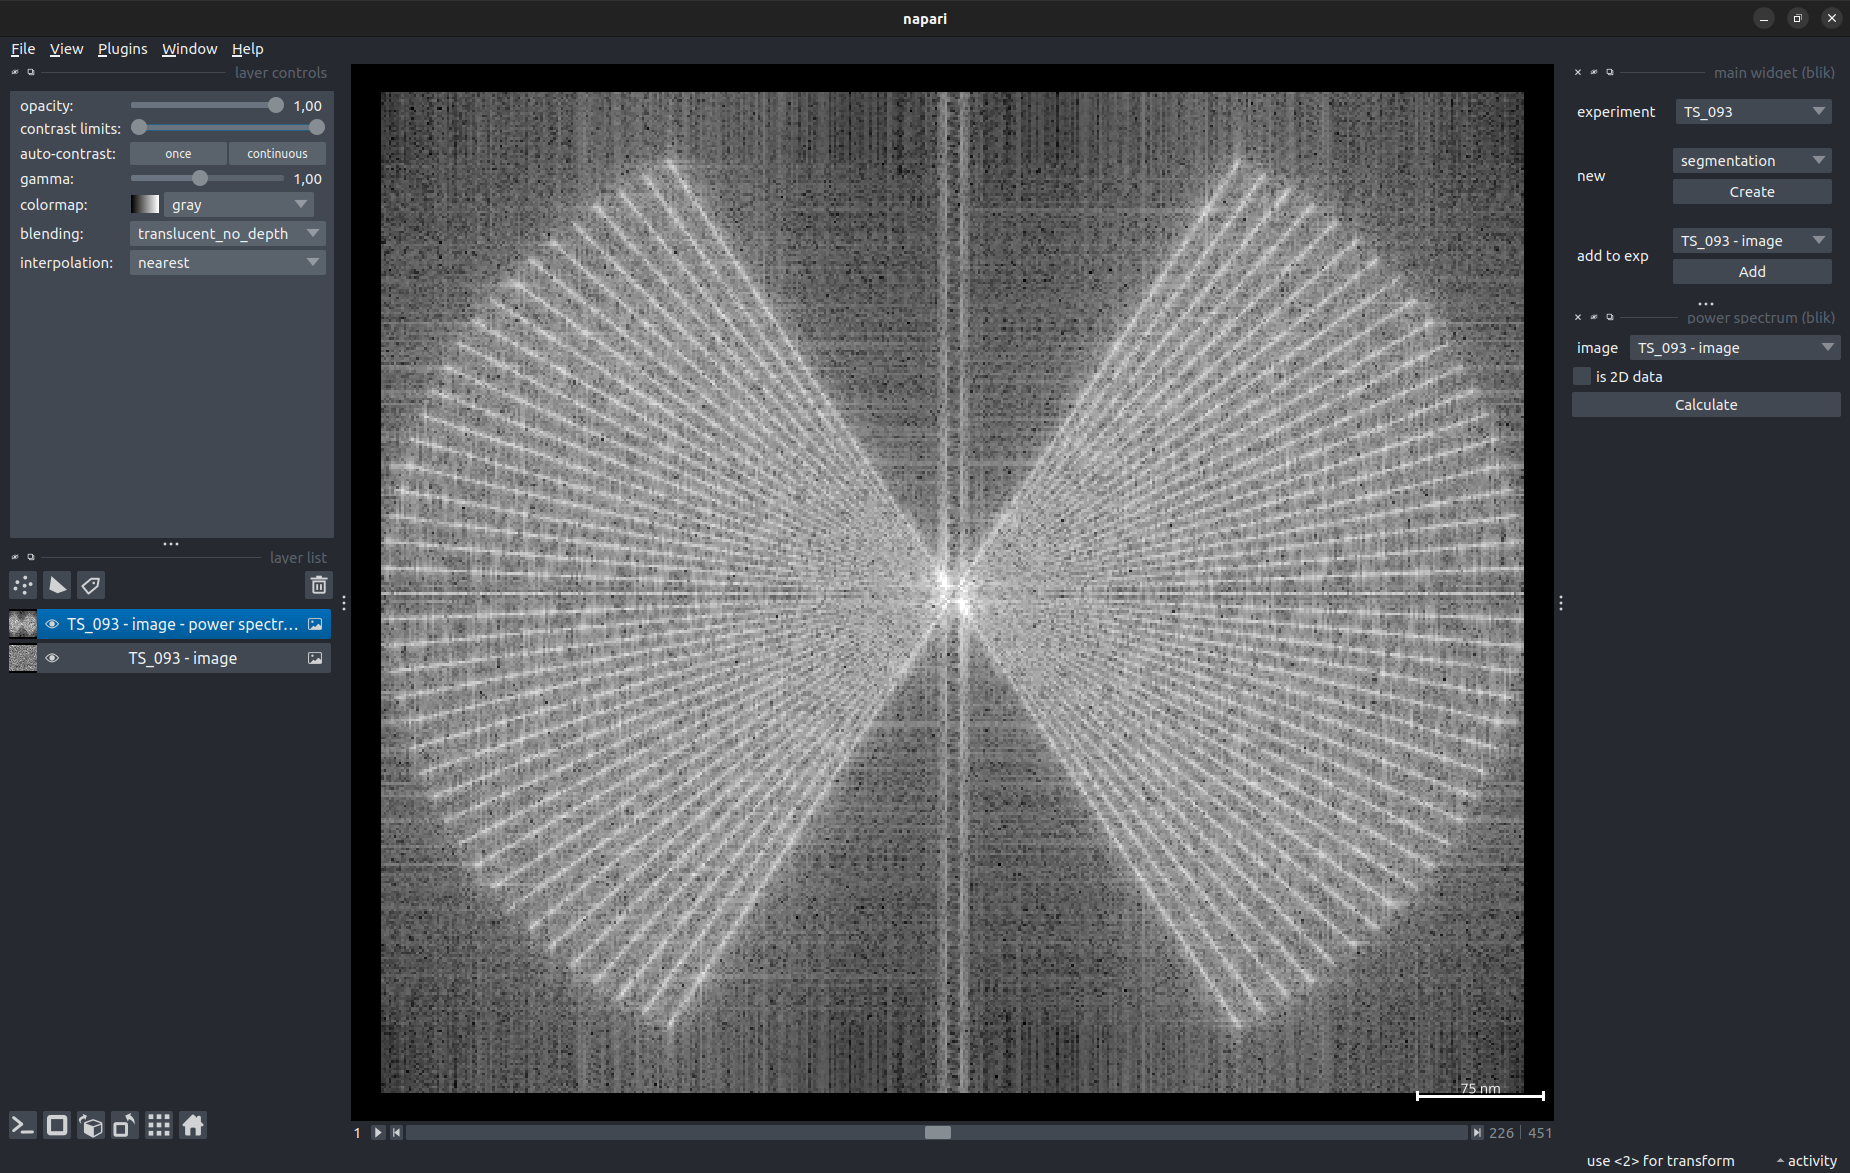
\includegraphics[width=\textwidth]{introduction/missing_wedge.png}
    \caption[Missing wedge]{2D slice through the 3D FT of a tomogram, perpendicular to the tilt axis. The 2D FT of images of the tiltseries are visible as lines at regular angular spacing; at the top and bottom they are not present, creating the missing wedge.}
    \label{fig:et_missing_wedge}
\end{figure}

\subsection{Annotation and segmentation}\label{et_annotation_segmentation}
Thanks to the \textit{in situ} and quasi-native nature of tomography data, it is often useful to annotate or segment tomograms in order to get a better view of the morphology of the sample, or to find areas and particles of interest more easily.

One of the most common approaches is to do semantic segmentation (aka labeling), where individual voxels are assigned a type --- "membrane", "ribosome", and so on, though usually in the form of a integer --- either by manually painting over the sample, or automatically via image processing algorithms or ML tools.
Labeling helps with visualisation by boiling down the sample to its most fundamental components, while also serving as a powerful tool for quantitative and morphological analysis of complex mesoscale objects.
To this end, segmentations are often used as starting point for other kinds of annotations, such as abstracting membranes or filaments to mathematical objects like splines and skeletons (CITE skan?) in order to calculate properties such as membrane curvature, filament branch length, and so on.

In some projects, morphology is all that matters, with no need to reach high resolution; in such cases, the cryo-ET pipeline can stop after annotation.
Where high resolution molecular structures are the goal, segmentations and other annotations may also be used as a starting point for particle picking.

\subsection{Particle picking}\label{et_particle_picking}
Picking particles in tomograms is not so different from picking particles from 2D micrographs, other than having an extra dimension.
Manual picking and template matching are still the preferred methods, though more and more software is developed for ML-based or hybrid methods (CITE cryolo, ...).

As with most things in cryo-ET, low SNR is the main obstacle to overcome; this is why some picking tools --- such as the one developed during this thesis (see \fullref{blik}) --- attempt to use as much prior knowledge about the system as possible in order to limit the degrees of freedom when searching for particles~\cite{castano-diezDynamoCatalogueGeometrical2017,wagnerEvolutionSPHIREcrYOLOParticle2020,gaifasBlikExtensible3D2024}.

Whenever possible, segmentation or other kinds of annotation can be used as baseline for particle picking: either by masking areas of interest --- such as picking only inside a certain cellular structure --- or by seeding particle picks based on the annotation geometry --- such as distributing particles on the surface of a membrane.
Such information may also be used to initialize the particle orientation to something self-consistent (e.g: all perpendicular to the membrane); this can affect drastically the initial model generation and subsequent refinement, where 3D rotational search may otherwise not overcome the SNR.

\subsection{Subtomogram averaging}\label{et_sta}
In cryo-ET, the equivalent to SPA's 2D classificatin and 3D refinement is subtomogram averaging (STA).
The idea at the core is the same: by combining the data from many subvolumes extracted from the tomogram (subtomograms) which contain copies of the same object, the SNR can be drastically improved.
The basic procedure is also very similiar to SPA, only in 3D: subtomograms are extracted from the full reconstructed tomogram based on the positions of the particle picks; then, rounds of cross-correlation and refinement (and/or classification) improve the model until convergence (see \fullref{em_classification}).

In recent years, however, the field is moving away from this simpler approach where "rigid" subtomograms are extracted from a full 3D reconstruction, in favor of directly reconstructing subtomograms from the 2D data, using what is sometimes called \textbf{per-particle tilt series}~\cite{zivanovBayesianApproachSingleparticle2022,tegunovRealtimeCryoelectronMicroscopy2019,chenCompleteDataProcessing2019}.
This opens up many avenues for optimization, such as 3D-CTF correction (see \fullref{et_tomo_reconstruction})~\cite{turonovaEfficient3DCTFCorrection2017}, multi-particle refinement~\cite{tegunovMultiparticleCryoEMRefinement2021}, bayesian polishing~\cite{zivanovBayesianApproachSingleparticle2022}, and more.


TODO: missing wedge effect on alignment

\subsection{Refinement}\label{et_refinement}

TODO: not sure if there's anything else to say here, maybe no need.

\subsection{Pros and Cons}
...

\newpage

\FloatBarrier

\begin{outline}
\1 Background on Cryo-EM in structural biology
    \2 \tick Base concepts (do not spend too much time on this)
        \3 \tick sample prep
        \3 \tick exposure damage
        \3 \tick role of detectors and resolution revolution \cite{faruqiCCDDetectorsHighresolution2000}
        \3 \tick data collection
        \3 \tick image formation
        \3 \tick CTF
        \3 \tick defocus (and ranges of defocus) and info spread
        \3 \tick dataset cleaning
        \3 \tick particle picking
        \3 \tick cross correlation
        \3 \tick 2D classification and selection
        \3 \tick typical processing steps, theory behind reconstruction and classification (more time here as it's more relevant for cryoet and my work)
        \3 \tick single particle analisys
        \3 \tick model building
    \2 \tick typical use cases (some example of single particle data, maybe using ftsz images) and advantages
        \3 \tick no crystal, simpler sample prep
        \3 \tick heterogeneity to a certain extent
        \3 \tick more native state
        \3 \tick bigger targets? complexes
    \2 \tick limitations (leading up to cryo-et) and comparison with other techniques (xray, nmr)
        \3 \tick sample prep/thickness/denaturation
        \3 \tick context missing
        \3 \tick ability to capture dynamics/heterogeneity (more/less than other techniques)
        \3 \tick Signal/Noise
\1 cryo-et, concepts and advantages
    \2 \tick base concepts and differences from SPA from thechnical standpoint
        \2 \tick cryoem, but different data acquisition and thus data processing
        \3 \tick exposure damage and dose issues
        \3 \tick sample prep (thinnes especially important because SNR)
        \3 \tick tilt-series alignment (fiducials), deformation, other aberrations, how they are tackled
        \3 \tick 3D CTF
        \3 \tick missing wedge, issues it introduces
        \3 \tick feature deletion (e.g: fiducials)
        \3 \tick segmentation/morphology
        \3 \tick STA (picking, averaging, classification, ...) for non-unique objects (template matching, geometric and template free, machin learning)
    \2 \tick some references/reviews (cool stuff you can do)
        \3 \tick \cite{turkPromiseChallengesCryoelectron2020,lucicCryoelectronTomographyChallenge2013}
    \2 what it provides compared to SPA
        \3 more native state and context preservation
        \3 single-particle insights
        \3 mesoscale and superstructural information
    \2 limitations (both in terms of technique, and in terms of current state of development)
        \3 (some mentioned before, maybe need to connect these two parts a bit better)
        \3 need for custom workflow cause the goal and problems are usually unique
        \3 issues caused by the missing wedge (alignement, reconstruction, interpretability)
        \3 SNR, denoising
        \3 visualisation/interaction
        \3 object identification (crowding
    \2 related techinques to overcome some limitations
        \3 FIB, what it enables and how it works
        \2 CLEM
\end{outline}
